\documentclass[11pt, letterpaper]{article}
\setcounter{tocdepth}{4}
\setcounter{secnumdepth}{4}
\usepackage[english]{babel}
\usepackage{fontspec}
\setmainfont{Times New Roman}
\usepackage{float}
\usepackage{tabularx}
\usepackage{adjustbox}
\usepackage{multirow}
\usepackage{longtable}
\usepackage{graphicx}
\usepackage{geometry}
\usepackage{xcolor,colortbl}
\usepackage{sectsty}
\usepackage{titlesec}
\usepackage{textcomp}
\usepackage{subfigure}
\usepackage{nameref}

\titleformat{\paragraph}
    {\normalfont\normalsize\bfseries}{\theparagraph}{0.2em}{}
\titlespacing*{\paragraph}{\parindent}{1.25ex }{1.75ex}

\sectionfont{\fontsize{18}{15}\selectfont}
\subsectionfont{\fontsize{16}{15}\selectfont}
\subsubsectionfont{\fontsize{14}{15}\selectfont}

\usepackage{enumitem}
\newlist{NH}{enumerate}{1}
\setlist[NH]{label=H\arabic*:}

\newlist{MN}{enumerate}{1}
\setlist[MN]{label=MN\arabic*:}

\newlist{MC}{enumerate}{1}
\setlist[MC]{label=MC\arabic*:}

\newlist{MP}{enumerate}{1}
\setlist[MP]{label=MP\arabic*:}

\usepackage{hyperref}
 \geometry{
    a4paper,
    total={170mm,257mm},
    left=20mm,
    top=25mm,
 }
 \hypersetup{
    colorlinks=true,
    linkcolor=black,
    filecolor=magenta,      
    urlcolor=blue,
}

\usepackage{fancyhdr}
\setlength{\headheight}{27.72354pt}
\addtolength{\topmargin}{-15.72354pt}
\pagestyle{fancy}
\usepackage{tikz}
\usetikzlibrary{automata, positioning, arrows}

\definecolor{maroon}{cmyk}{1,0,1,0.6}

\begin{document}

    \begin{titlepage}
        \begin{center}
        \vspace*{1cm}
            \begin{figure}
                \centering
               
\includegraphics[width=10cm]{images/logos/Logo_Politecnico_Milano.png}
            \end{figure}
            
            \huge
            \textbf{Usability Report on The Intern Group website}

            \vspace{1cm}
        
            \Large
            \textbf{Hypermedia Applications}

            \vspace{1.5cm}

            \begin{figure}[H]
                \centering
                
\includegraphics[width=9cm]{images/logos/i3lab.png}
            \end{figure}

            \vspace{2cm}

            \begin{tabular}{c|c}
                Student & Person Code\\
                \hline\hline
                Davide Di Marco & 10667065\\
                Stefano Fossati & 10569836\\
                Davide Maffi & 10630074\\
                Marco Romanini & 10613151
            \end{tabular}
            \large
            
        \end{center}
    \end{titlepage}

\cleardoublepage

\fancyhead{}
\fancyfoot{}
\fancyhead[L]{Usability Report}
\fancyhead[C]{}
\fancyhead[R]{Di Marco Davide, Fossati Stefano, Maffi Davide, Romanini Marco}
\cfoot{\thepage}

\tableofcontents
\cleardoublepage

%%%
\section{Abstract}

In this document, we present and discuss the usability evaluation of the website \href{https://www.theinterngroup.com/}{“the Intern Group” }, a website offering the possibility to apply for global and virtual internships around the world. \\
The main goal of the analysis is to investigate the usability issues and concerns faced by using the website, from the perspective of experienced and inexperienced users. Then, this report is supposed to give guidelines and clues to the client for a redesign activity of the product, in order to improve its overall usability.  
\\ \\
The evaluation has been divided in two parts, using two complementary methods: Expert Evaluation (or Inspection) and User Testing. 
\\
The aim of the Expert Evaluation, performed by the team members, is to judge the usability of the website, according to a set of predefined heuristics. In this way, we are able to give a complete overview of the product. 
\\
The aim of the User Testing, instead, is to provide a fresh and non-expert point-of-view of the website, concerning common and relevant interactions with the product. This evaluation is performed by an external group of people, who represent a sample of the actual users that are likely to use the website. 
\\ \\
The results of both parts have then been used to derive final conclusions and considerations about the product, in order to provide useful feedback. 


\section{Experts Evaluation}
\subsection{Introduction - Methodology}
 Experts inspect websites with the help of Heuristic-based techniques.
These heuristics have been used to analytically review UX-related elements of an application and determine whether specific website features comply with a set of quality requirements.
Nielsen and MiLe have been used as heuristics.
The Nielsen ones were our initial choice because they are the most common and can evaluate the entire website.
The MiLes are instead, structured heuristics that concentrate on particular elements of the website during analysis, such as the text font, layout, or coherence of the visual aspects. 

\subsubsection{Heuristics}
\paragraph{Nielsen Heuristics}
\begin{NH}
    \item  Visibility of system status. \\
            “The system should always keep users informed about what is going on, through appropriate feedback within reasonable time”.
    \item Match between system and the real world. \\
            “The system should speak the users' language, with words, phrases and concepts familiar to the user, rather than system-oriented terms. Follow real-world conventions, making information appear in a natural and logical order”.
    \item User control and freedom. \\
            “Users often choose system functions by mistake and will need a clearly marked "emergency exit" to leave the unwanted state without having to go through an extended dialogue. Support undo and redo”.
    \item Consistency and standards. \\
            “Users should not have to wonder whether different words, situations, or actions mean the same thing. Follow “platform” conventions”. 
    \item Error prevention. \\
            “Even better than good error messages is a careful design which prevents a problem from occurring in the first place. Either eliminate error-prone conditions or check for them and present users with a confirmation option before they commit to the action”.
    \item Recognition rather than recall. \\
            “Minimize the user's memory load by making objects, actions, and options visible. The user should not have to remember information from one part of the dialogue to another. Instructions for use of the system should be visible or easily retrievable whenever appropriate”.
    \item Flexibility and efficiency of use. \\
            “Accelerators --unseen by the novice user-- may often speed up the interaction for the expert user such that the system can cater to both inexperienced and experienced users. Allow users to tailor frequent actions”.
    \item Aesthetic and minimalist design. \\
            “Dialogues should not contain information which is irrelevant or rarely needed. Every extra unit of information in a dialogue competes with the relevant units of information and diminishes their relative visibility”. 
    \item Help users recognize, diagnose and recover from errors.  \\
            “Error messages should be expressed in plain language (no codes), precisely indicate the problem, and constructively suggest a solution”.
    \item Help and documentation. \\
            “Even though it is better if the system can be used without documentation, it may be necessary to provide help and documentation. Any such information should be easy to search, focused on the user's task, list concrete steps to be carried out, and not be too large“.
\end{NH}

\paragraph{MiLe Heuristics}
\begin{MN}
    \item Interaction consistency: \\
            Do pages of the same type have the same links and interaction capability? 
    \item Group navigation: \\
            Is it easy to navigate from and among groups of “items”? E.g. From the “list of items” of a group to its “members” (and the other way around); among different “groups”; among members of the same group (next/previous). 
    \item Structural Navigation: \\
            Is it easy to navigate among the “components” (parts) of a topic?
    \item Semantic Navigation:  \\ 
            Is it easy to navigate from a topic to a related one (in both directions)? 
    \item “Landmarks”: \\
            Are “landmarks” useful to reach the key parts of the web site?
\end{MN}
\vspace{1cm}
\begin{MC}
    \item Information overload: \\
            Is the information in a page too much/too little? 
    \item Consistency of Page Content Structure:  \\
            Do pages of that present topics of the same category have the same types of elements?
\end{MC}
\vspace{1cm}
\begin{MP}
    \item Text layout: \\
            Is the text readable? Is font size appropriate? 
    \item Interaction placeholders-semiotics: \\
            Are textual or visual labels of interactive elements “expressive”? i.e. do they reflect the meaning of the interaction and its effects? Are they consistent? 
    \item Interaction placeholders-consistency: \\
            Are textual or visual labels of interactive elements consistent in terms of wording, icon, position, etc.?
    \item Spatial allocation: \\
            Is the on-screen allocation of contents and visual appropriate for their relevance? Are “semantically related” elements close and “semantically distant” elements far away? 
    \item Consistency of Page Spatial Structure: \\
            Do pages of the same type have the same layout (same visual properties of each component and similar organization and lay-out of the various elements?
\end{MP}

\subsubsection{Evaluation criteria}
Each heuristic has been evaluated with a score from 1 to 5 where: 
\begin{enumerate}
    \item unusable, heuristic not respected.
    \item heuristic not always respected, presents many problems.
    \item heuristic respected but has some errors.
    \item heuristic respected but still has few errors.
    \item heuristic respected without any errors.
\end{enumerate}

\subsection{Approach}
Before the individual expert evaluation, the whole team had superficially surfed the website in order to understand the main aspect of the system. The main target of the application is detected to be the university’s students, a minor target are applicants and workers. The target website is an informative website that contains information about the possibility of an internship organized by Intern Group. We had considered to insert a constrain on the minimum number of pages that each team member has to inspect, based on the analysis of the main pages and the web structure. \\
This superficial analysis helped in the defining of the individual inspection process work as following:
\begin{itemize}
    \item The inspector has to surf the website for at least 3h. In this way we are almost sure that the different inspector uses the site three time more than a common user session. During the remaining time the inspector is free to navigate the website as he prefers.
    \item The main sub-pages must be navigated. In particular, the Career Fields, the destinations and who-you-are pages. This decision was taken because these pages contain the main contents in which a common user is interested in.


\end{itemize}

\subsection{Results}

\subsubsection{Table of results}

\begin{table}[H]
    \centering
    \begin{tabularx}{1\textwidth} { 
        | >{\centering\arraybackslash}X 
        | >{\centering\arraybackslash}X 
        |  c
        | >{\centering\arraybackslash}X | }
        
    \hline
    \rowcolor{maroon!55}
    Category & Code & Heuristics & Score \\
    \hline
    Navigation & H1  & Visibility of system status & 3 \\
    \hline    \rowcolor{maroon!30}
    Presentation & H2 & Match between system and the real world & 4 \\
    \hline
    Navigation & H3 & User control and freedom & 3 \\
    \hline    \rowcolor{maroon!30}
    Presentation & H4 & Consistency and standards & 4 \\
    \hline    
    Presentation & H5 & Error prevention & 3 \\
    \hline    \rowcolor{maroon!30}
    Navigation & H6 & Recognition rather than recall & 4 \\
    \hline    
    Navigation & H7 & Flexibility and efficiency of use & 3 \\
    \hline    \rowcolor{maroon!30}
    Presentation & H8 & Aesthetic and minimalist design & 2 \\
    \hline    
    Presentation & H9 & Help users recognize, diagnose and recover from errors & 4 \\
    \hline    \rowcolor{maroon!30}
    Content & H10 & Help and documentation & N/A \\
    \hline    
    Navigation & MN1 & Interaction consistency & 4 \\
    \hline    \rowcolor{maroon!30}
    Navigation & MN2 & Group navigation & 4 \\
    \hline    
    Navigation & MN3 & Structural Navigation & 4 \\
    \hline    \rowcolor{maroon!30}
    Navigation & MN4 & Semantic Navigation & 4 \\
    \hline    
    Navigation & MN5 & Landmarks & 4 \\
    \hline    \rowcolor{maroon!30}
    Content & MC1 & Information overload & 4 \\
    \hline    
    Content & MC2 & Consistency of page content structure & 5 \\
    \hline    \rowcolor{maroon!30}
    Presentation & MP1 & Text Layout & 5 \\
    \hline    
    Presentation & MP2 & Interaction placeholders-semiotics & 4 \\
    \hline    \rowcolor{maroon!30}
    Presentation & MP3 & Interaction placeholders-consistency & 4 \\
    \hline    
    Presentation & MP4 & Spatial allocation & 4 \\
    \hline    \rowcolor{maroon!30}
    Presentation & MP5 & Consistency of Page Structure & 4 \\
    \hline
    
    \end{tabularx}
\end{table}

\subsubsection{Detailed results}
In this section every heuristic used will be elaborated further in order to explain why that score was given and what errors/good things have been found.

\paragraph{Presentation Heuristics}
\begin{enumerate}
    \item[H2)] Match between system and the real world. 
        \begin{itemize}
            \item The "Who you are" label in the menu has some ambiguous item in the drop-down menu.  
            \item In the "How it works" label is pretty unclear what the next-step refers to (see the highlight button on Figure ~\ref{fig:H2}). As an user I would expect other words to find program alternatives.
            \item Overall the website tends not to use technical language, so that the navigation among the pages isn't so difficult even for non-expert users.
            \item The menu bar is very useful and lets the user orientate easily. Even the item in the drop down menu express straight forward what they will contain.
            \begin{figure}[H]
                    \centering
                    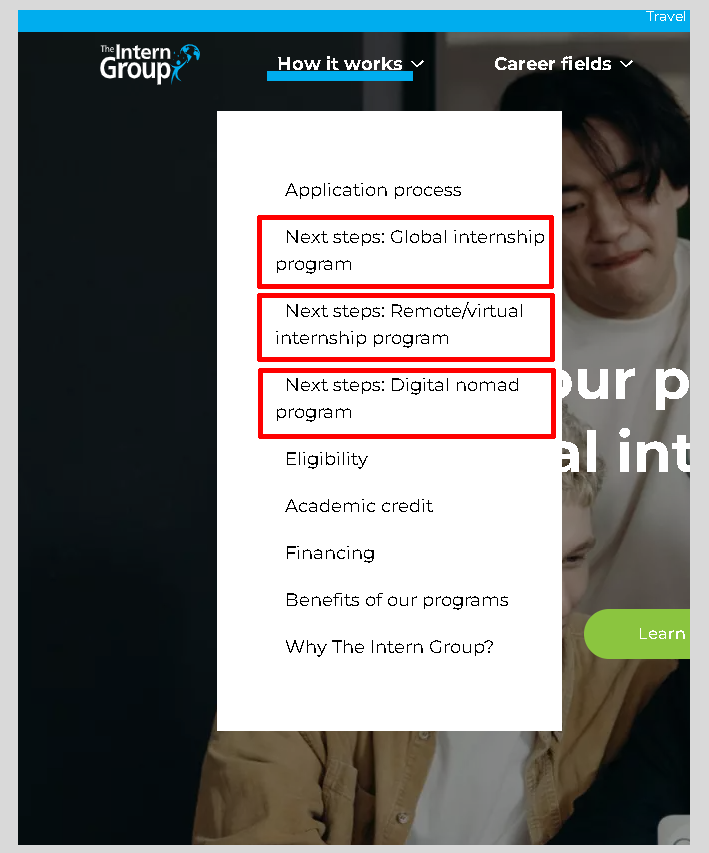
\includegraphics[width=6cm]{images/inspection/H2.png}
                    \caption{The menu linked to the "how it works" button.}
                    \label{fig:H2}
                \end{figure}
        \end{itemize}
        \item[H4)] Consistency and standards.
            \begin{itemize}
                \item Clicking on the "who you are" button in the upper menu brings the user to a page that is structured in subpages. However, these are different from those in the drop-down menu which appears when the user passes over the same button. Also, it is not clear where the user will be brought when clicking on the "who you are" button in the upper menu.
                \item Standards are overall respected (menus are placed on the top and often on the left of the pages, contact info are placed at the bottom right corner of the pages, the logo is top left and links to the home page). However there are some minor consistency issues (the "high school student" personal info form is placed differently from the other forms, the "recruit interns" page doesn't have the upper menu anymore, sometimes the Location Based Bread Crumbs are not clickable).
                \begin{figure}[H]
                    \centering
                    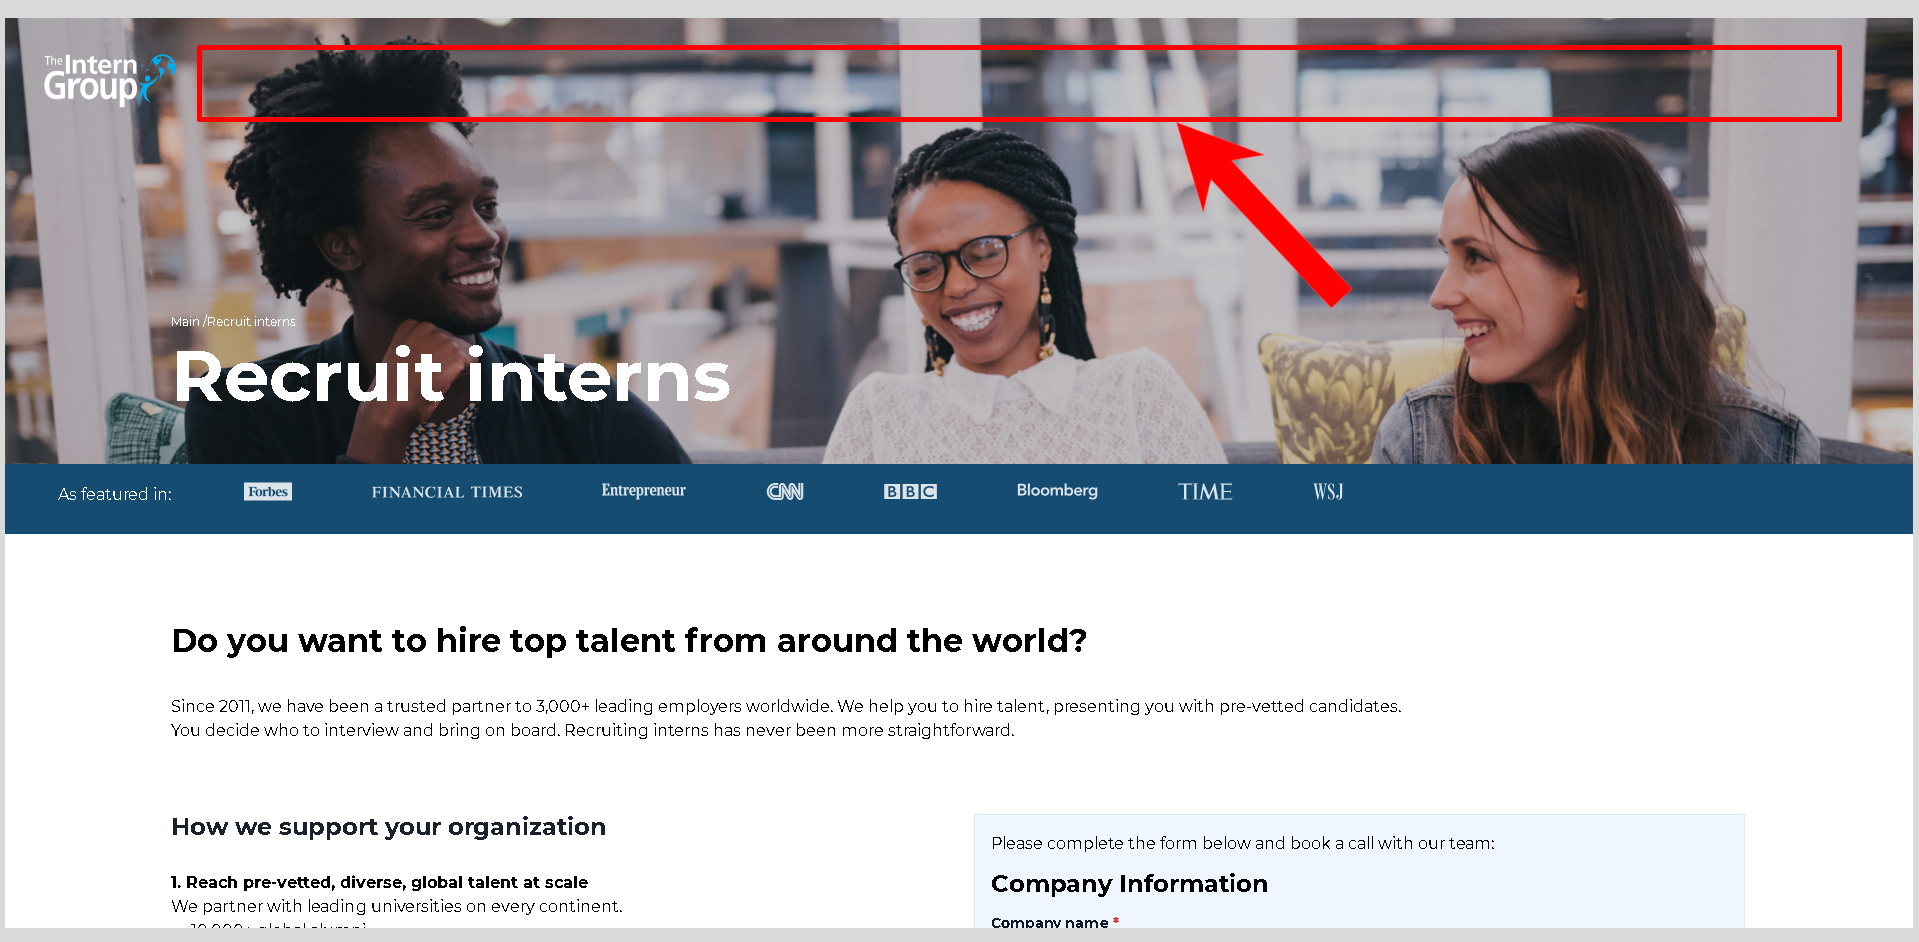
\includegraphics[width=10cm]{images/inspection/H4_1.png}
                    \caption{In this page the menu is missing (in the red rectangle).}
                \end{figure}
            \end{itemize}
        \item[H5)] Error prevention.
            \begin{itemize}
                \item The Apply Now filling page has a lot of controls on the data format (like email) and for other entries ha a list of possible choices with an example format under, in order to avoid possible mistakes.
                \item The "Contact us" pop up on the right also has checks on the email formats.
                \item There are some pages that exists but as soon as you try to get more info clicking on them, they lead to an empty page (IT internship in Milan).
                \item A useful tool if the filter in the "Career Fields" page, the problem is that selecting some of them (for example the "medical electives and public health" filter) produces zero results. 
                \begin{figure}[H]
                    \centering
                    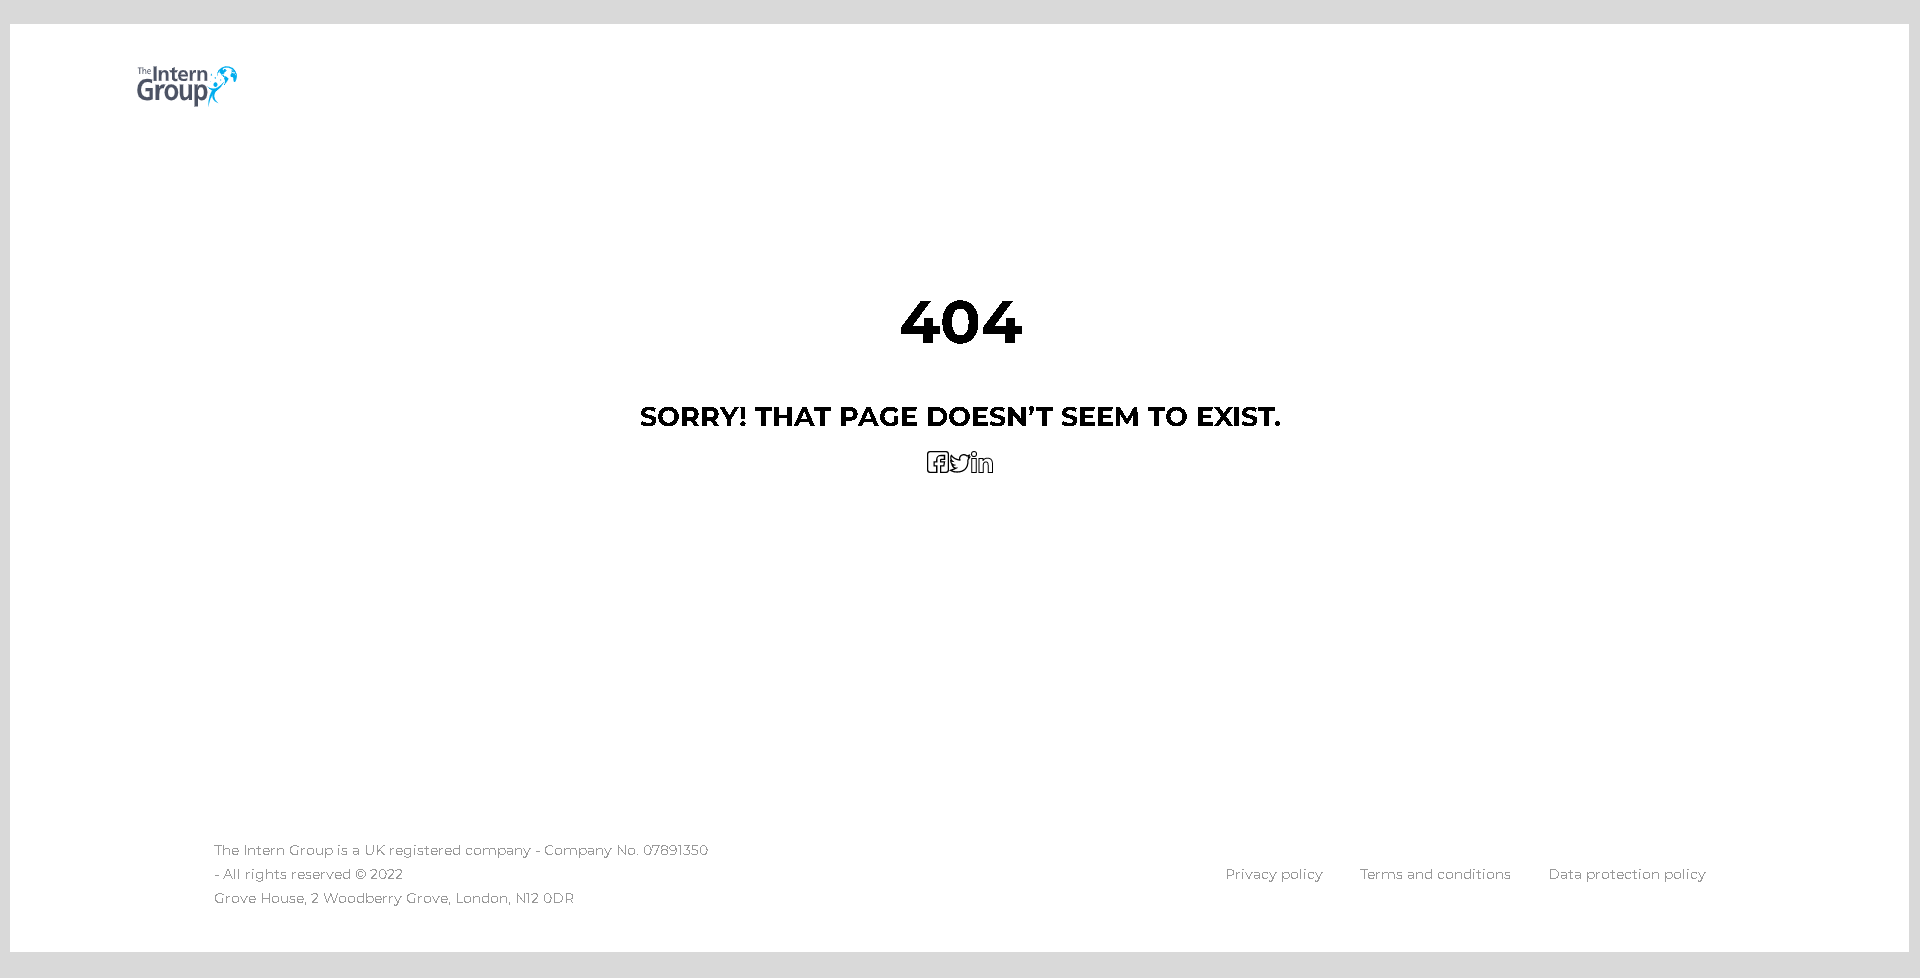
\includegraphics[width=8cm]{images/inspection/H5.png}
                    \caption{The error page that is visualized by the user in case of wrong link or missing page.}
                \end{figure}
            \end{itemize}
        \item[H6)] Recognition rather than recall.
            \begin{itemize}
                \item The upper menu navigation is full enough to help the user reach the majority of the pages in the website.
                However, some pages are not accessible from a direct navigation of the ones in the same category, but are reachable only through links placed inside pages of other categories: this means that reaching again a specific page may require a memory effort to recall exactly its location. In addition, the website provides us some pages structured with left menus and some other not. This lack forces the user to memorize the exact location in a specific page of the information or of the link connected to other pages. 
                \item The Apply Now and the filter at the bottom of the home page form uses some sliding menu in order to help the user in the element selection. 
                \begin{figure}[H]
                    \centering
                    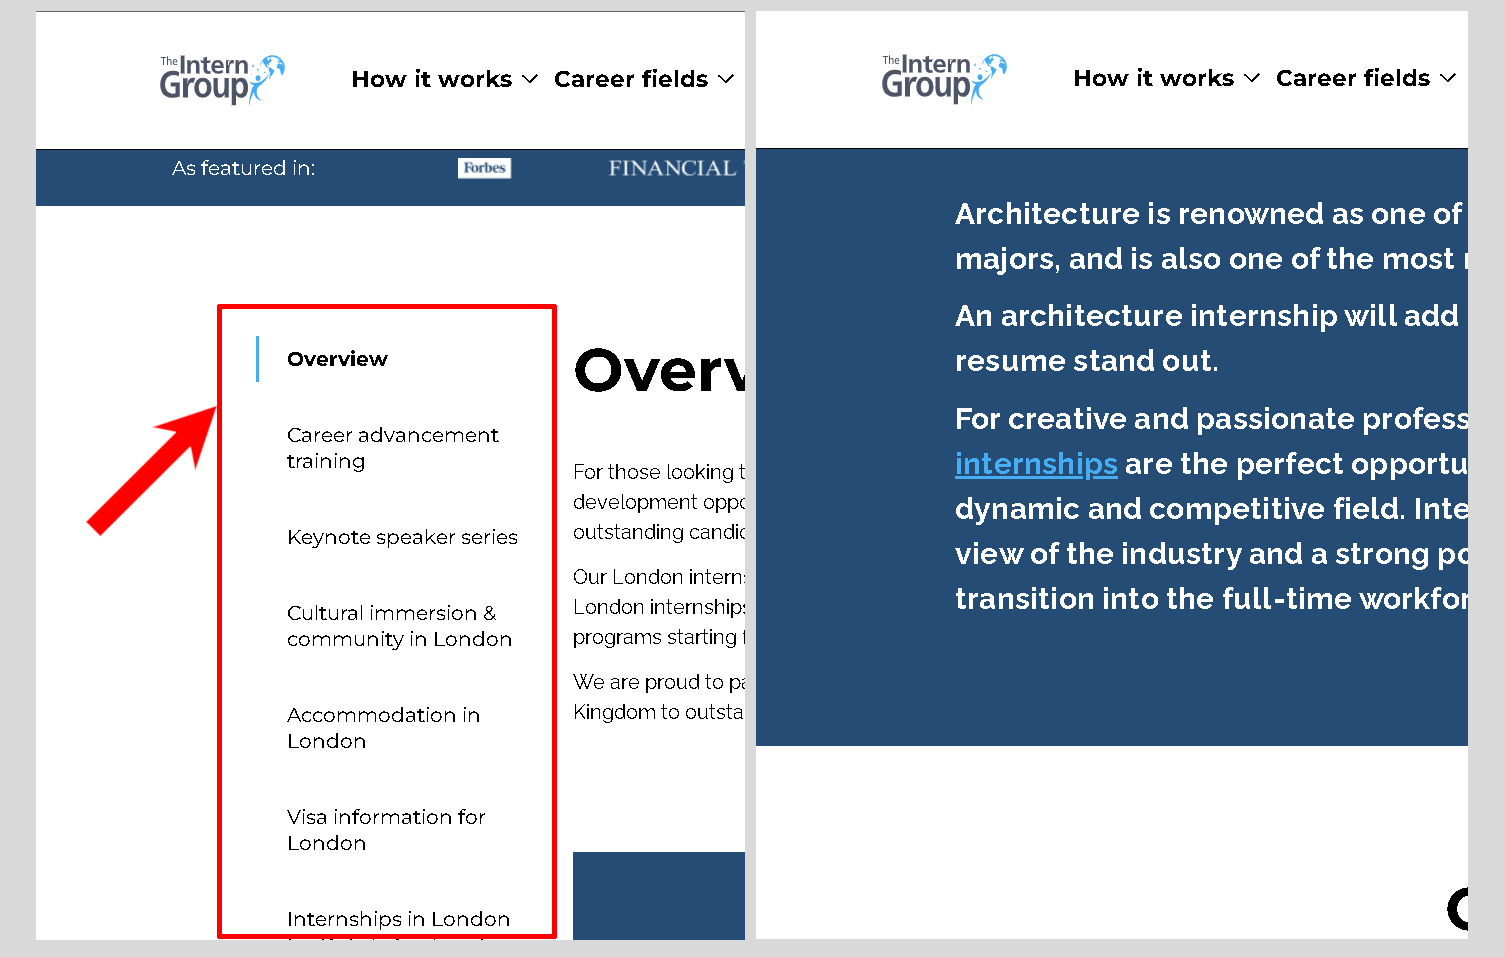
\includegraphics[width=10cm]{images/inspection/H6.png}
                    \caption{On the left the structured page of London "destination", on the right the non-structured page of the Architectural "career field". (in realtà piu che unstructured  è non navigabile tramite il menu}
                \end{figure}
            \end{itemize}
        \item[H8)] Aesthetics and minimalist design.
            \begin{itemize}
                \item The amount of text is well balanced. However, there are too many large images displayed almost everywhere: they are just annoying to scroll every time just to reach the useful information. Moreover, there are many redundant elements repeated in certain groups of pages (such as the generic "Our programs" section in all the "Career fields" pages) that could at least be reduced in size, if not simply removed, given the fact that they have their own easily reachable page. Moreover, there are many menu and links which is not minimalist. Once you browse to a page on the menu you can reach a wall of text where you can get lost.
                \begin{figure}[H]
                    \centering
                    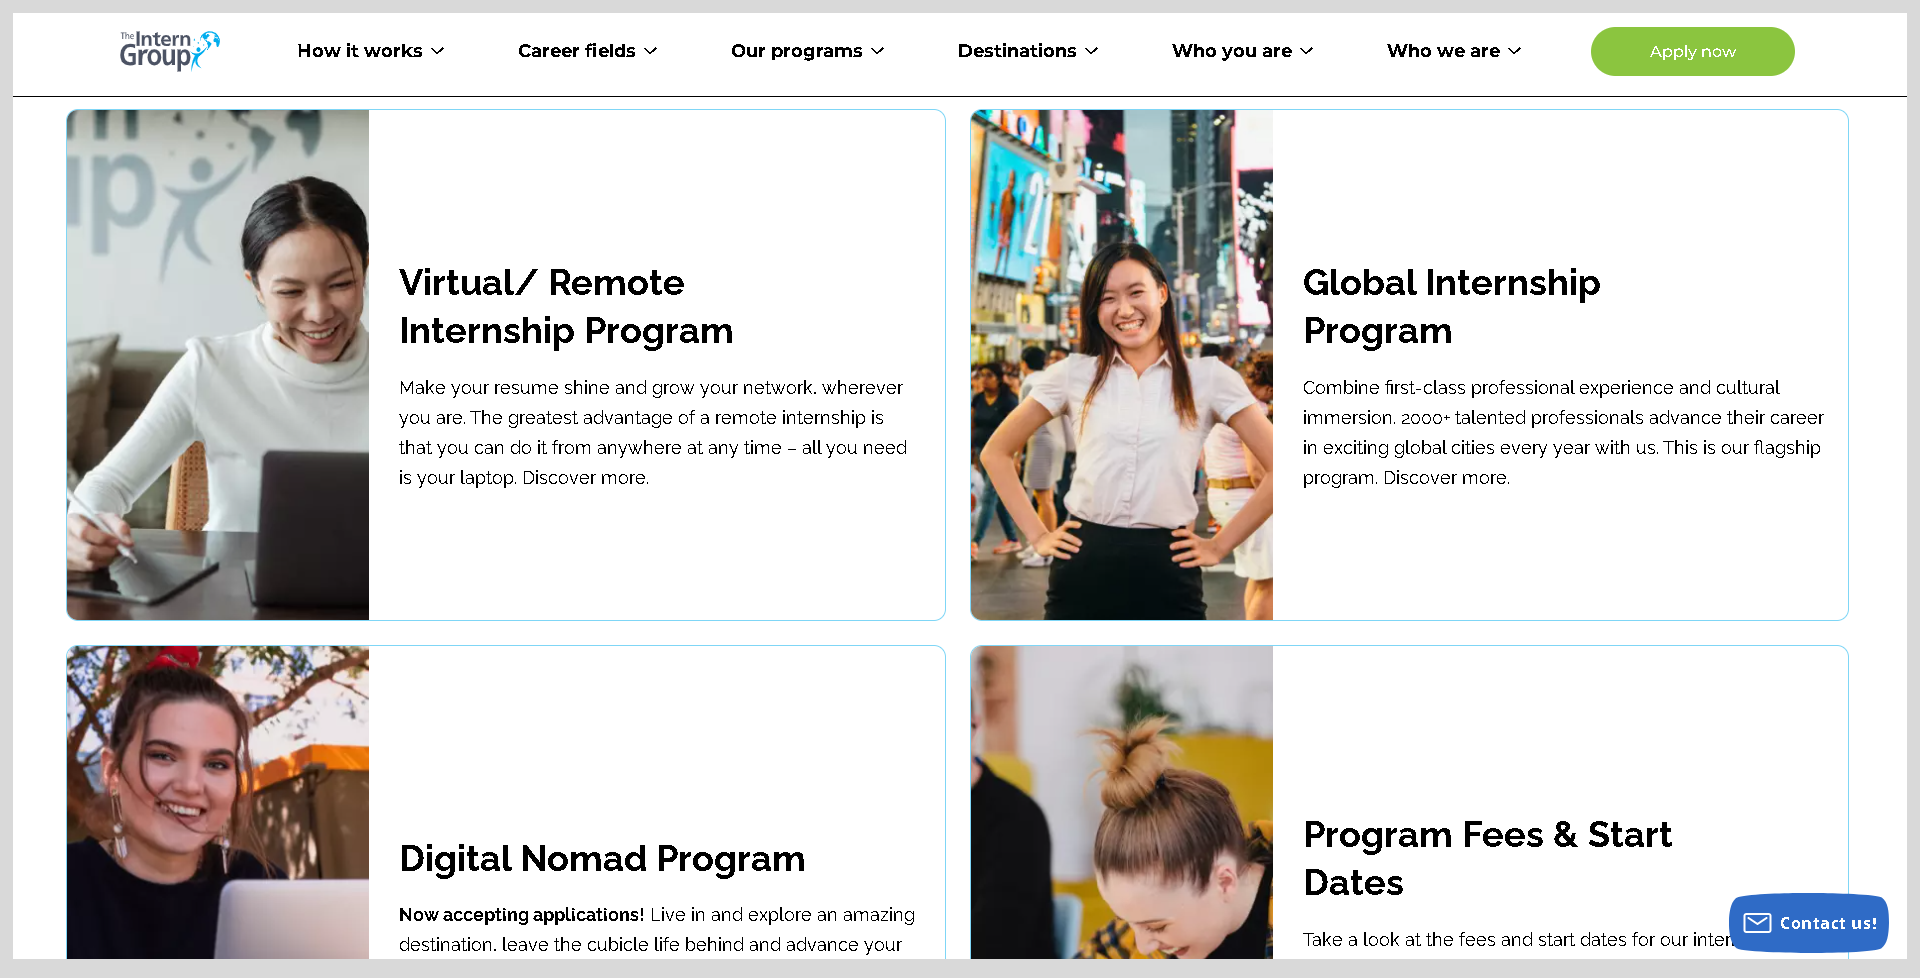
\includegraphics[width=10cm]{images/inspection/H8.png}
                    \caption{This screen shows a part of page that is present in the all the career filed pages and other ones. This element is repetitive everywhere and is not needed in some pages.}
                \end{figure}
            \end{itemize}
        \item[H9)] Help users recognize, diagnose and recover from errors. 
            \begin{itemize}
                \item There are no particular user-input sections, apart from subscription to the newsletter, inserting personal info in the "Who you are" section and applying for an internship. The most part of this forms are sufficiently supported by error messages in case mandatory information is missing or not correct. The website presents few links to non-existent pages and the system shows an error page that don’t display a clear button or input for go back to the previous page. The only visible element is the logo that can be used to go to the home page. 
            \end{itemize}
        \item[MP1)] Text Layout.
            \begin{itemize}
                \item The text is very readable, and the font size is well balanced except for some breadcrumbs.
            \end{itemize}
        \item[MP2)] Interaction placeholders-semiotics.
            \begin{itemize}
                \item The interactive elements are "intuitive": the textual and visual labels for interactive elements convey their functional meaning.
            \end{itemize}
        \item[MP3)] Interaction placeholders-consistency.
            \begin{itemize}
                \item The main menu is composed only by words.
                \item In some of the pages accessible from the main menu, the button to navigate inside pages of the same topic is not easily visible. The "previous" button is grey, so it seems not to be clickable while it is. Another example could be the "load more" button.
                \item Some link to other page are hidden inside a little "here" hyperlink.
                \item The visual elements are consistent: in pages of the same type they have the same visual properties.
            \end{itemize}
        \item[MP4)] Spatial allocation.
            \begin{itemize}
                \item  The layout of the elements and their relevance are handled quite well in most pages, except for some elements that are inserted in many pages with a too generous size compared to their relevance for those pages. In addition, the page structure is such that the elements are grouped together at spatial level when they are semantically close together.
            \end{itemize}
        \item[MP5)] Consistency of Page Spatial Structure.
            \begin{itemize}
                \item All "Career fields" pages are structured the same way even though to get some information a user has to scroll through the whole page since there isn't a logical thread that the pages follow. Same goes for the Destinations page.
                \item The Page Spatial Structure between pages of the same type is overall consistent. However, a little exception is, for instance in "Who you are", between different pages of this sub-menu (particular case "high school student"), personal info form is placed sometimes at the bottom of the page, while for other categories of users it is placed at the top of the page.
                \item If we take into account page different from destinations, on the left side appears a menu to navigate pages of the same topic. Menu that is not present in the destinations pages.
                \begin{figure}[H]
                    \centering
                    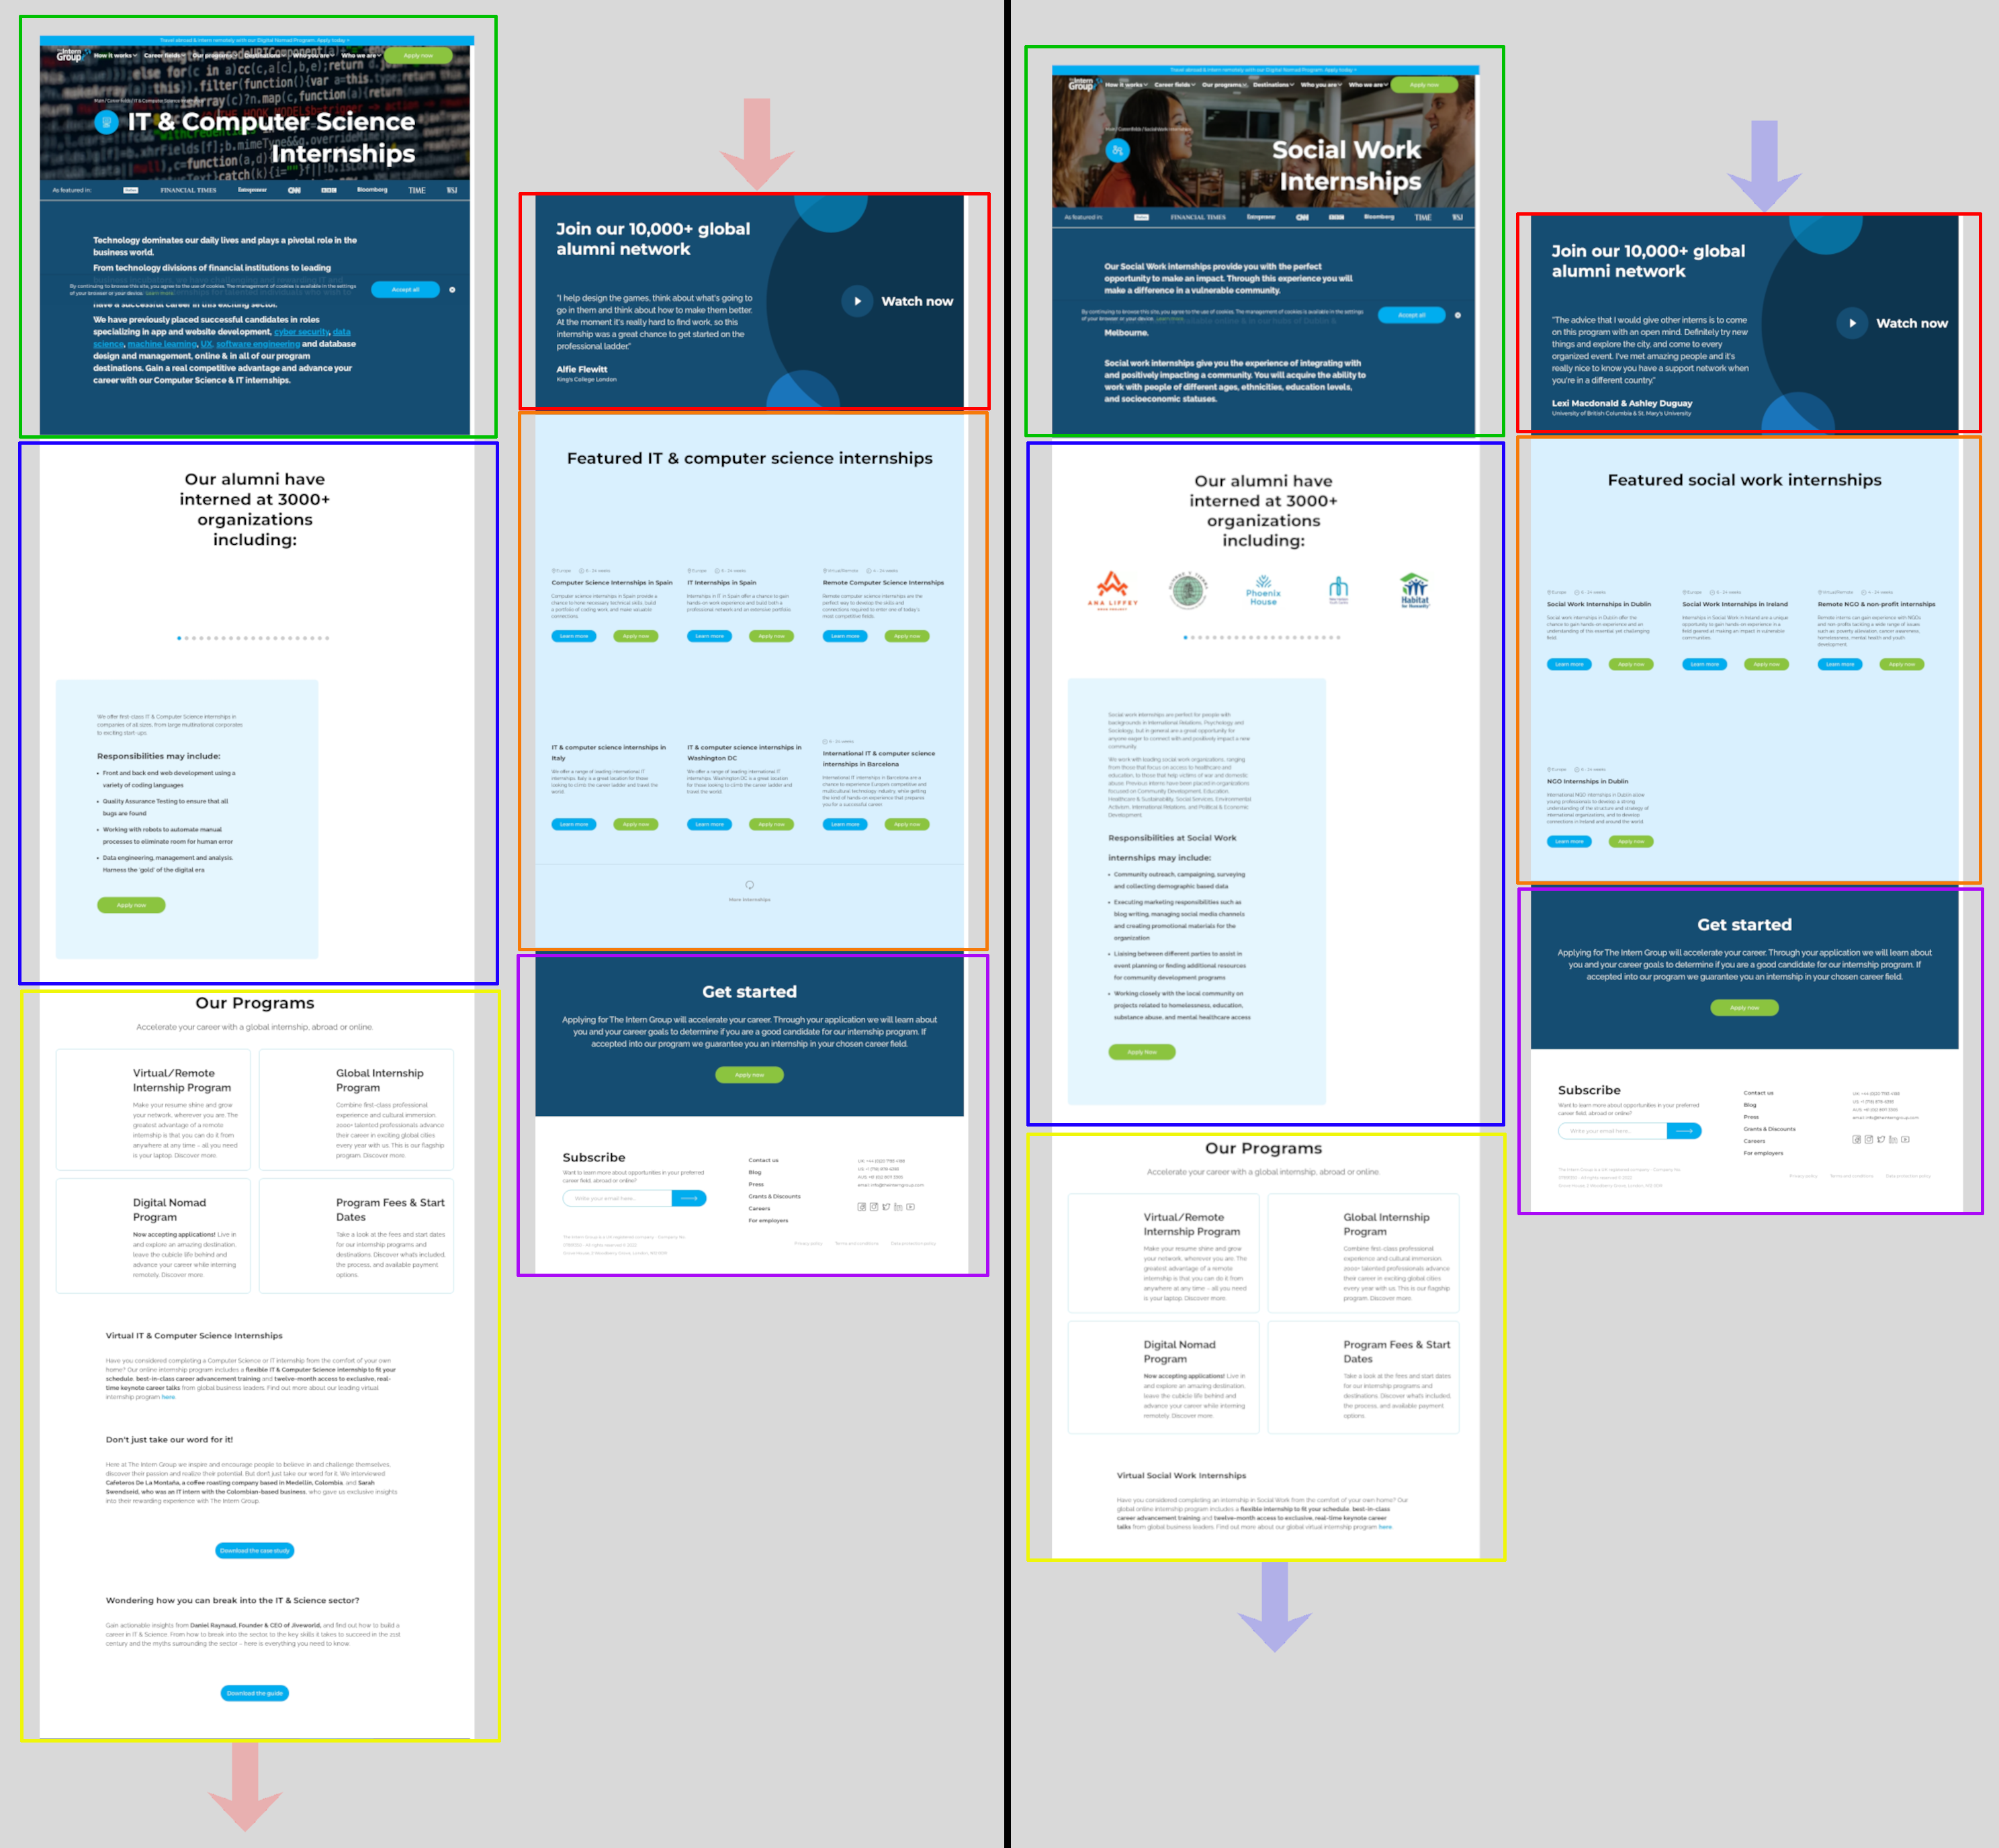
\includegraphics[width=12cm]{images/inspection/MP5.png}
                    \caption{The images shows two different "career field" full pages (one on the right of the black line and one on the left). The pages have the same consistent structure. The same part of the related page is circled with the same color}
                \end{figure}
            \end{itemize}     
\end{enumerate} 

\paragraph{Navigation Heuristics}
    \begin{enumerate}
        \item[H1)] Visibility of system status.
            \begin{itemize}
                \item The Path is not always present and, even when it's present, it's in a very little font and with a color that merges with the background.
                \item The left-side menu helps the navigation through pages within the same topic.
                \begin{figure}[H]
                    \centering
                    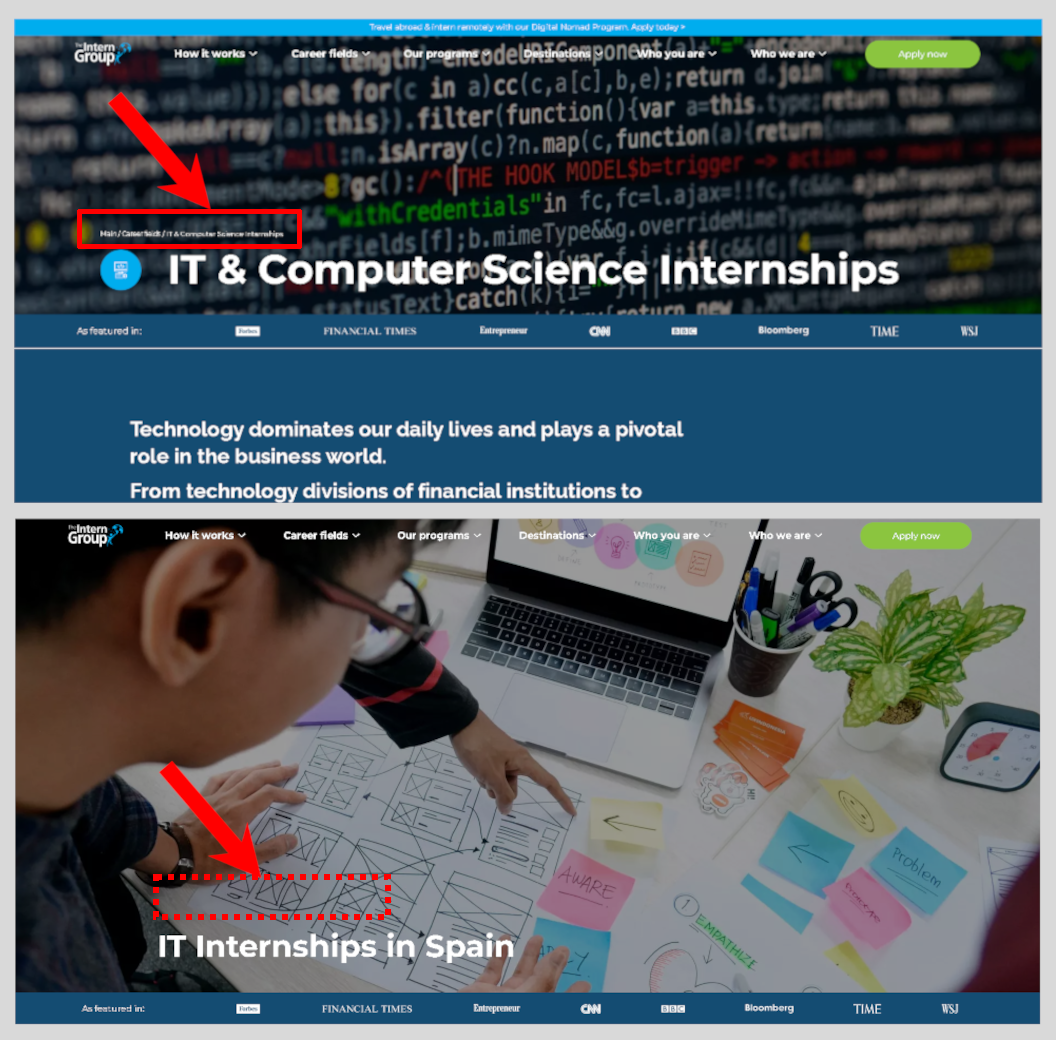
\includegraphics[width=8cm]{images/inspection/H1.png}
                    \caption{The image above shows a page of career field with its little path. The image below shows another part of the website where the path is not present}
                \end{figure}
            \end{itemize}
        \item[H3)] User control and freedom.
            \begin{itemize}
                \item Logo always present so that the user can always come back to the home page.
                \item Since this is mainly an information site, there isn't the need to exit big procedures. What is missing is some sort of "back button" (besides the one of the browser), otherwise the only alternative is starting again from the upper menu and reach again the previous destination. For example: following the path "Career fields -> Engineering" and going to Learn more, if i got here by mistake there's no way of going back if not re-doing the same path over again.
            \end{itemize}
        \item[H6)]
            \begin{itemize}
                \item The upper navigation menu is full enough to help reaching the majority of the pages in the site. However, some pages are not accessible from a direct navigation of the ones in the same category but are reachable only through links placed inside pages of other categories: this means that reaching again a specific page may require a memory effort to recall exactly its location. In addition, the website provides us some pages structured with sub-menus and some other not. This lack obliges the user to memorize the exact location in a specific page of the information or of the link connected to other pages. 
                \item The Apply Now and the filter at the bottom of the home page form uses some sliding menu in order to help the user in the element selection. 
            \end{itemize}
        \item[H7)]
            \begin{itemize}
                \item The site is mainly an information site, and for that purpose is quite efficient to navigate. The upper menu, however, is maybe overcrowded with links, at the point that some drop-down menus must be scrolled to find the right link or may occupy the entire screen. Some grouping in macro-categories could have been done to be able to navigate more quickly the upper menu, which is the core navigation tool of the site. The menu is always visible and it’s a landmark increase the efficient of use.  
                \item In the other hand some pages are not structured with sub-menus, this lack don’t help the user to be efficient in finding specific information. 
            \end{itemize}
        \item[MN1)] Interaction consistency.
            \begin{itemize}
                \item The interaction possibilities are overall consistent, except sometimes for minor issues (e.g., Environmental Sciences \& Sustainability career field doesn't have clickable Bread Crumbs, or the upper menu in the "Recruit interns" page is missing). 
                \item In general, pages of the same section have the same types of links, so that the interaction possibilities are overall coherent. However, there are pages with basically the same content, which are physically different pages: this may cause some consistency issue. 
            \end{itemize}
        \item[MN2)] Group navigation.
            \begin{itemize}
                \item For the navigation between "Career Fields" or "Who you are" entries
                you must go back to the main menu.
                \item Group navigation is fine. However, the "previous/next" buttons could be more visible, while the upper menu creates a bit of Cognitive Overload, since it's very crowded with elements. 
            \end{itemize}
        \item[MN3)] Structural Navigation.
            \begin{itemize}
                \item There is no useful navigation tools inside "Career fields", you must read the whole page in order to retrieve information you need.
                \item In pages different from "Career fields" the Structural navigation is pretty good, mainly helped by the left-side menu, which is available in those pages that talk about different aspects of the same topic (e.g. destinations, programs).
            \end{itemize}
        \item[MN4)] Semantic Navigation.
            \begin{itemize}
                \item Let's suppose we're looking for Fashion Design in London. The user has two ways to get to the design location:
                \begin{enumerate}
                    \item Destinations \textrightarrow{} London \textrightarrow{} left menu on the entry Featured internship in London \textrightarrow{} manually look for the information needed.
                    \item Career fields \textrightarrow{} Fashion Internships \textrightarrow{} scroll down and find all the options available.
                \end{enumerate}
            \item To retrieve information about the eligibility with regards to the previous point, the path is also different. While in the first point we could find those info in the left menu, in the second one there's a small hyperlink at the end of the page.
            \item There are often inside the text some "semantic links" which redirect the user to useful pages, but they are almost never bidirectional. In general, however, the semantic connections are quite good: each "career field" page has links to both programs and related destinations, each "destination" page has links to available career internships, and many other useful links for other types of info
            \end{itemize}
        \item[MN5)] Landmarks.
            \begin{itemize}
                \item The menu is always present to help user navigation (only few sites make an exception like: "Became a host Organization", "Hire Interns" and "Apply now" since it opens another page). Same goes for the logo that leads to the homepage.
                \item The upper menu is the main landmark of the site and works fine. However, the Environmental Sciences \& Sustainability career field page doesn't have clickable bread crumbs, and the upper menu in the "Recruit interns" page is missing for no particular reason (as exposed previously in other comments).
                \item Some pages has literally wall of text that make the search of information a bit hard. But in the overall inside each page those Wall of text are separated by some images or other elements so that the page is well balanced. 
                \begin{figure}[H]
                    \centering
                    
\includegraphics[width=14cm]{images/inspection/MN5.png}
                    \caption{The images shows the menu (in red) that is always present during the navigation, and the logo (in blue) that is linked to the homepage}
                \end{figure}
            \end{itemize}
    \end{enumerate}
    
\paragraph{Content Heuristics}
    \begin{enumerate}
        \item[H10)] Help and documentation.
            \begin{itemize}
                \item There's no documentation that helps use the website, if any other information that is not on the website is needed, the user could always use the "Contact us" pop-up on the right or even the basic contact information on the bottom of each page.
            \end{itemize}
        \item[MC1)] Information overload.
            \begin{itemize}
                \item The amount of information displayed overall is well balanced, without becoming overwhelming. Very often the information is well structured, useful and concise. This is a crucial aspect, giving the fact that this mainly an information site (the only exception is made by the "Who you are" entries, since has way to many information among which the user has to orientate).
            \end{itemize}
        \item[MC2)] Consistency of Page Content Structure.
            \begin{itemize}
                \item Page Content Structure is overall consistent: all the pages of the same type have the same elements inside.
                \item Pages of the same topic adhere to the concept they're talking about. 
            \end{itemize}
    \end{enumerate}

\subsubsection{Conclusions}

\begin{figure}[H]
    \centering
    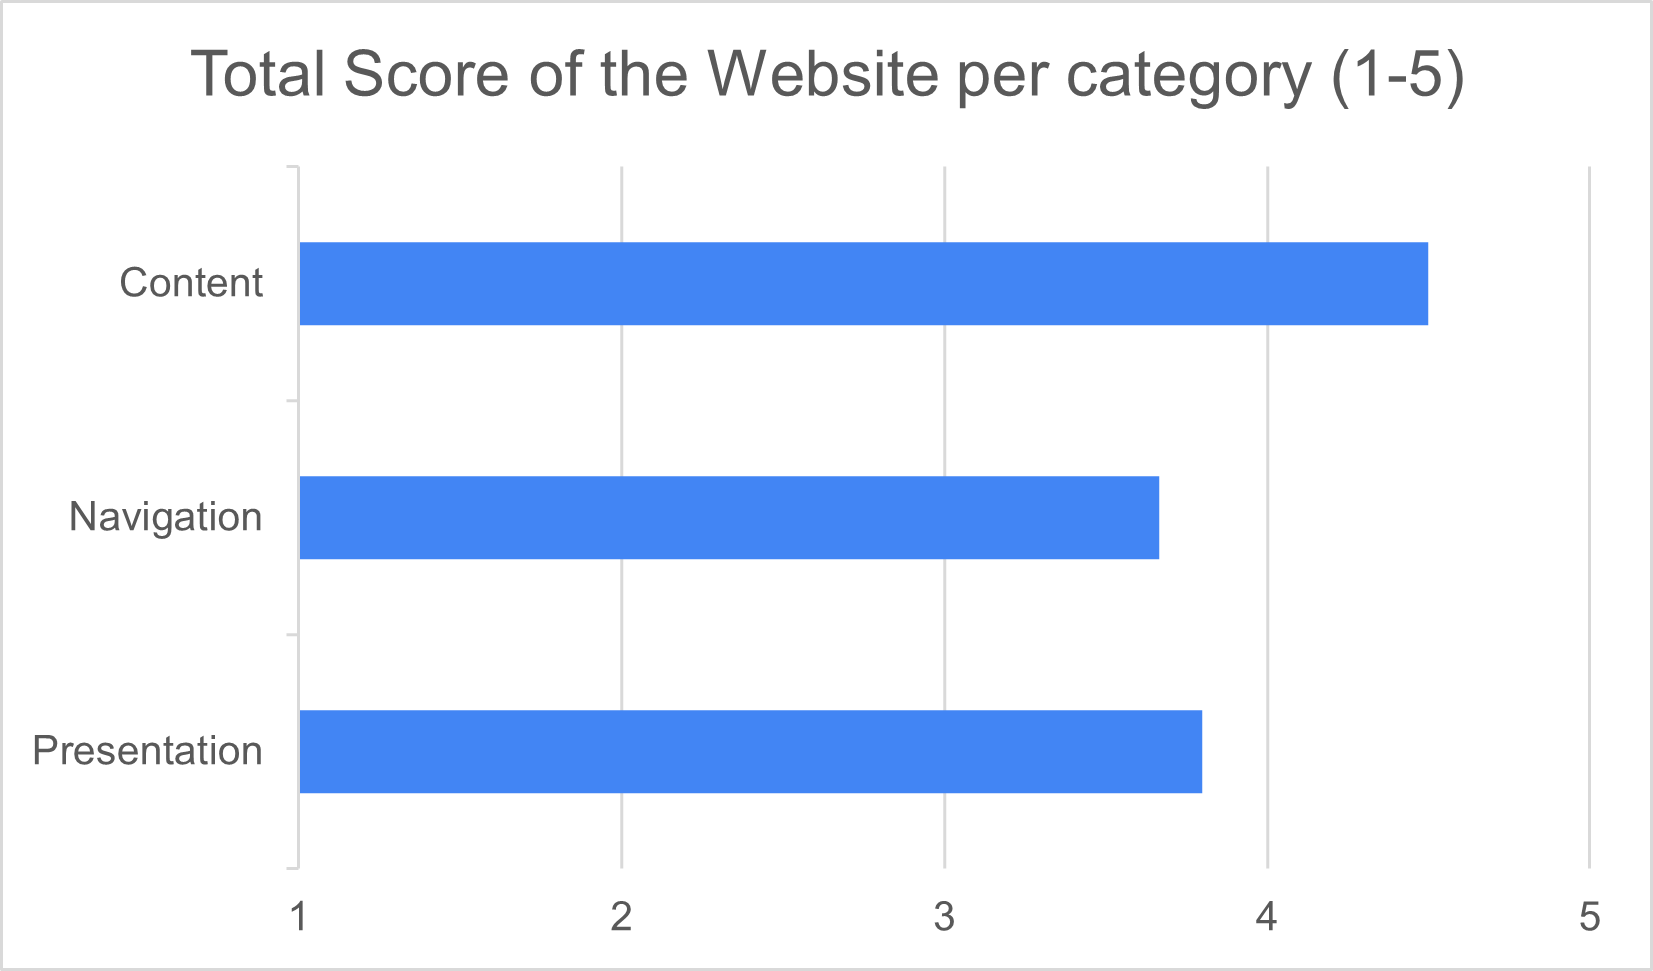
\includegraphics[width=8cm,height=4cm]{images/inspection/Conclusions/Category_score.png}
    \caption{Score based on the category}
    \label{fig:category_score}
\end{figure}

None of the categories evaluated achieved extremely low grades. In particular, as can be seen from \ref{fig:category_score}, the highest result was achieved by the category of contents that was evaluated through three heuristics. Instead, the navigation category has turned out the worst and the presentation one has been estimated with a rating slightly higher than the navigation one. Both of these latter categories have been evaluated through more than seven heuristics.

Analyzing specifically the evaluation of the navigation heuristics we can see that there is no heuristic completely respected and the heuristics H1, H3, H7 are just enough. In fact, we have generally encountered problems with the site in the navigation of some subgroups of the pages that were a bit 'cumbersome and do not always keep the user updated on where he is browsing. Instead, on the other navigation heuristics are almost always respected except in some exceptions, just as we have seen in the heuristic MN5 of the landmarks that are always present.

The presentation heuristics have less homogeneous evaluations than those of navigation; in fact, as it can be seen in \ref{fig:presentation_evaluations}, the heuristic H8 presented many problems and the heuristic H5 barely reached the sufficiency. In particular, the aesthetics of the pages must be improved because they have so many large elements that make them extremely long and are not displayed well. Even the presentation of error pages should be improved so as to allow the user to understand well what happened. However, note of merit for MP1 that obtained the highest score, in fact the text is always well readable and in an informative site this is an important aspect.

\begin{figure}[H]
    \centering
    \subfigure[Navigation Evaluations]{
        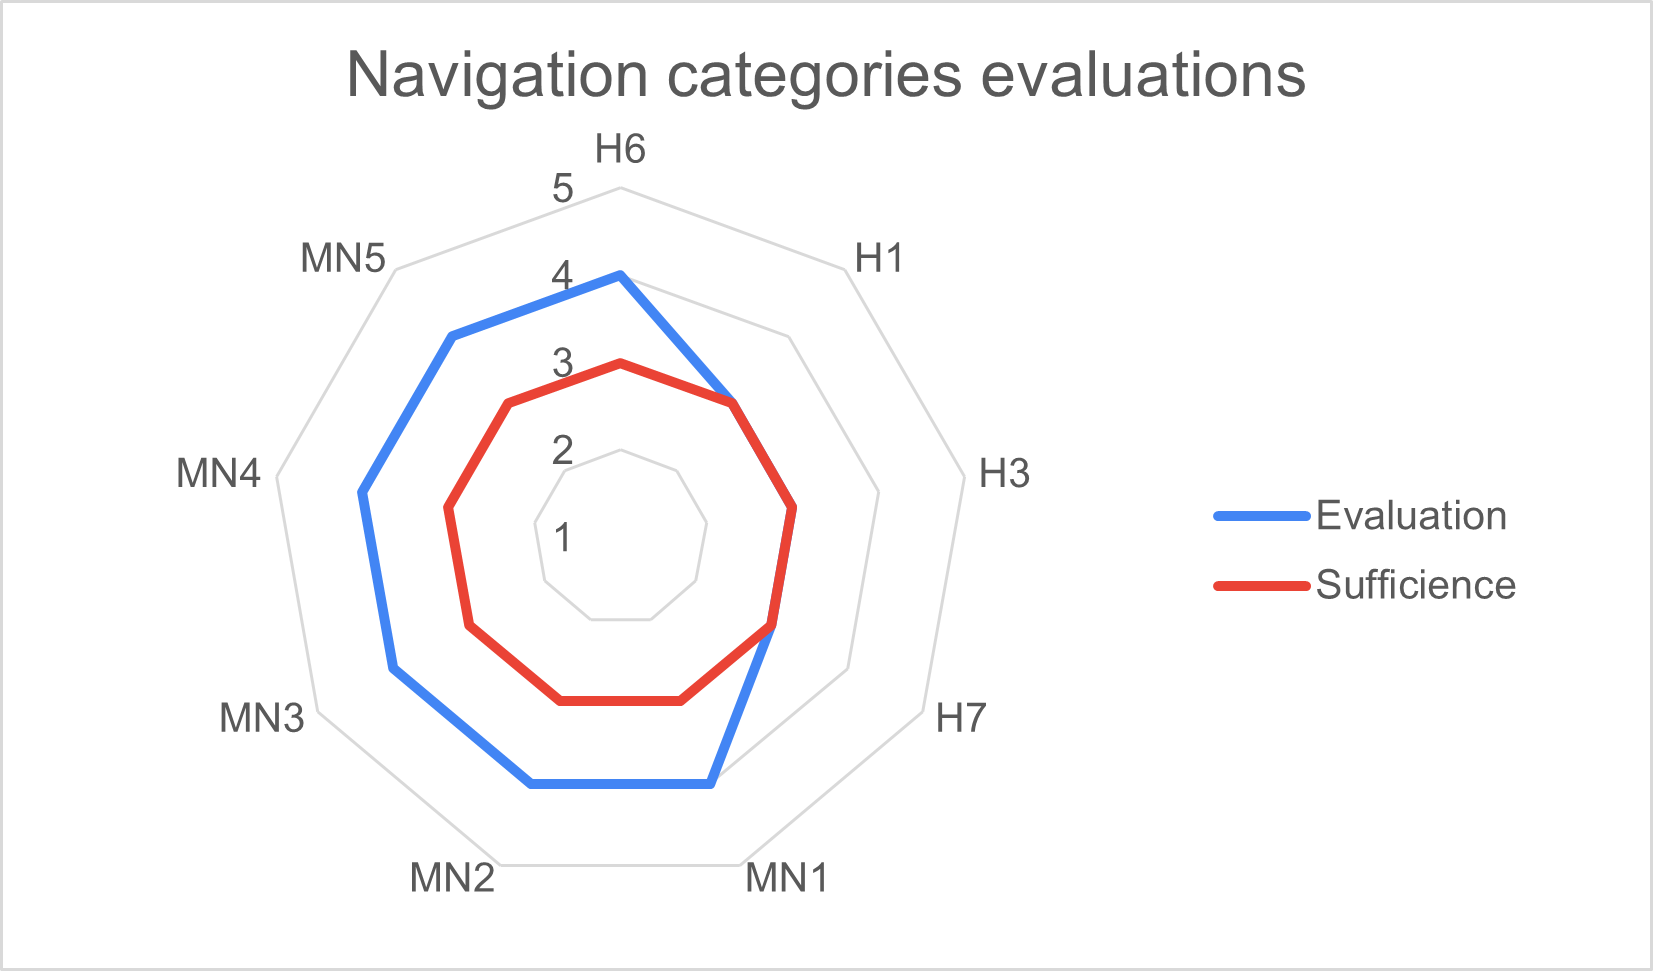
\includegraphics[width=8cm]{images/inspection/Conclusions/Navigation_evaluation.png}
        \label{fig:navigation_evaluations}
    }
    \subfigure[Presentation Evaluation]{
        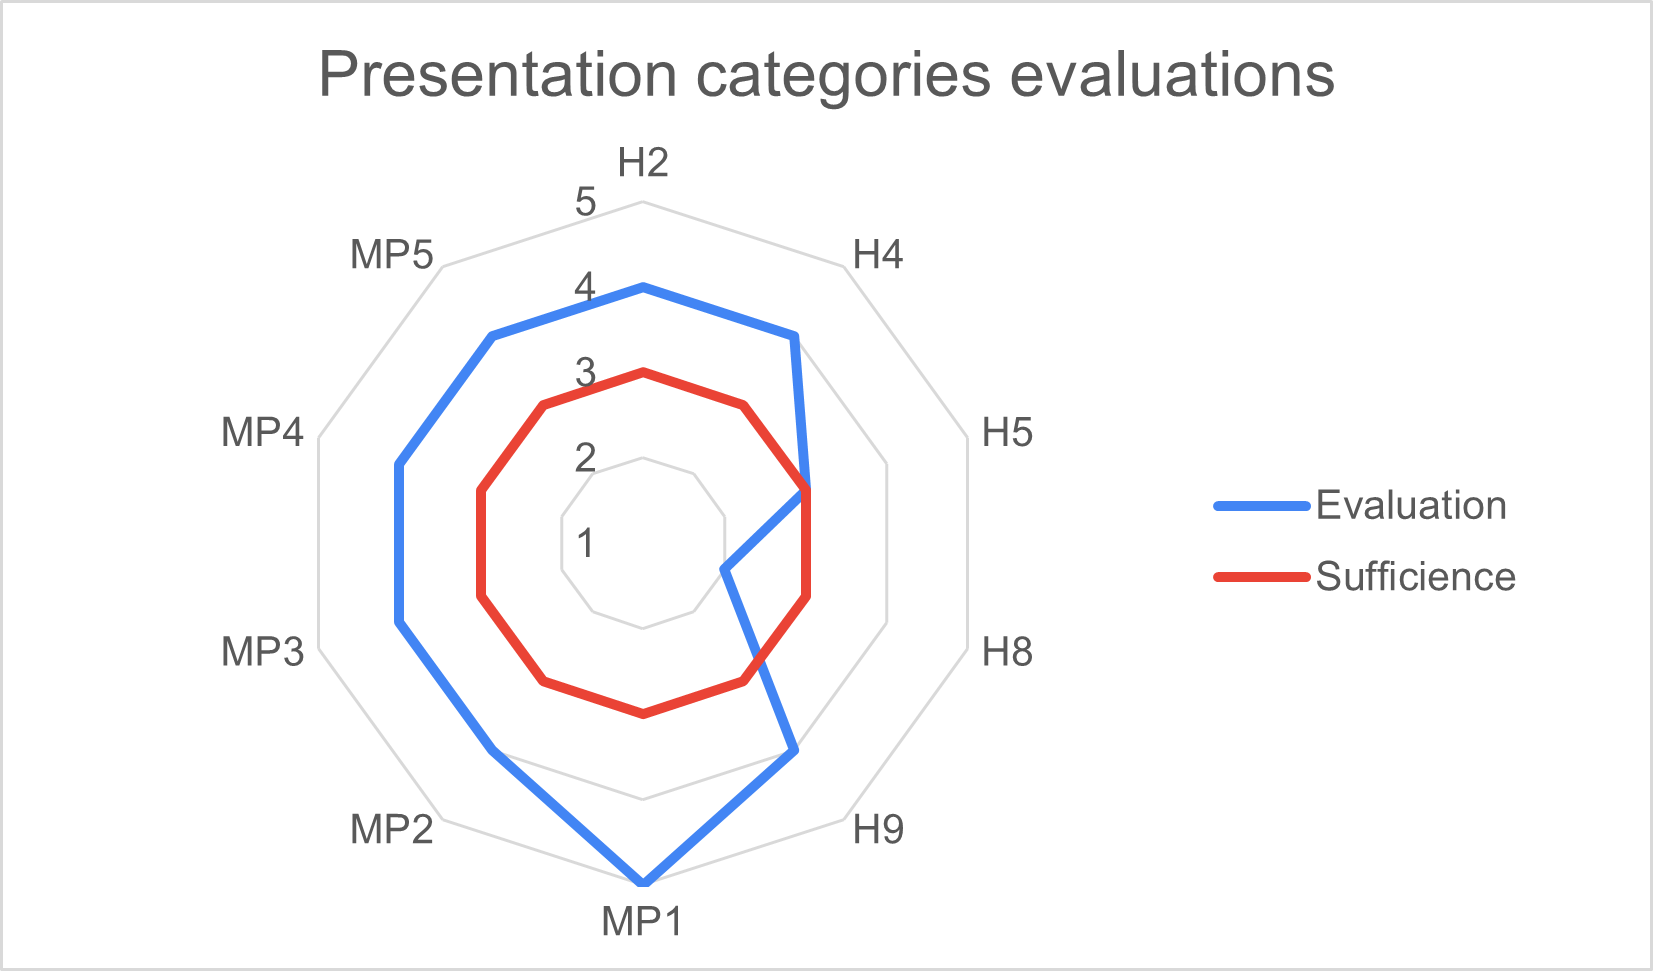
\includegraphics[width=8cm]{images/inspection/Conclusions/Presentation_evaluation.png}
        \label{fig:presentation_evaluations}
    }
    \caption{Categories evaluations}
\end{figure}

\newpage

\section{User Testing}
\subsection{General Method}
The main objective of User Testing is to obtain feedback from real common users about the usability of the website, as to enrich the analysis performed by the experts during the Inspection. In order to do so, a representative sample of potential target users must be gathered to perform the test: by observing their interactions and behaviours with the website, it is possible to derive deeper considerations about the product. \\
In this way, in fact, it is possible to detect certain kind of issues which were not found during the Inspection phase, or that were not perfectly caught using the heuristics approach.  \\
At the same time, User Testing can also be useful to validate or discard some of the judgements which have been made during the Inspection, depending on the effects they had on an actual usage of the site.  \\
Moreover, users may provide important info about the seriousness of previously detected errors and problems: an aspect which most users get stuck on will get more attention and have a higher priority than others which many users were easily able to overcome. 

\subsection{Study Design}
\subsubsection{User Selection and Recruiting}
The first step of the process is to select the sample of users. Given the fact that the website is about internships, we decided to conduct the User Testing study mainly on young people that are wondering to enter in the labour market, because we think they are the most common type of users that will access the platform. \\
For this reason, our class of analysis is composed by university students in the range of 20-27 years of age, with heterogeneous backgrounds and academic carriers. \\
Since the Nielsen Curve suggests that 5 users should be enough to detect about 85\% of the problems and 15 users should discover all of them, we selected 20 people to perform our test. For our small study, the users were recruited via direct connections and were not promised any compensation. 

\subsubsection{Tasks}
The tasks assigned to the users aim at representing a realistic usage of the website: they try to reflect actions and goals that a real user may be willing to perform or achieve. Some of them try also to analyse the behaviours of the users concerning specific issues that have been found in the Inspection phase. In general, they cover all the main sections of the website. \\
We decided to give the tasks to the users in random order, avoiding any logical link, rather than in a specific sequence. This was meant to minimise the learning capability of the users, as an attempt of analysing the website features with a point-of-view as objective as possible. For this reason, we shuffled the tasks and prepared different orderings for different users (they can be found in figure \ref{annex:task_sequence} of the annex section). We made sure that each task was the starting one exactly two times, so that each of them could be tested with no previous knowledge of the site. \\
\\
Here it follows the list of predefined tasks. There is also a brief description of the reasons and motivations for which we decided to use these tasks. Some of them are generic activities that aim at simply analyse common actions, while others try to focus on small problems that were previously detected. \\

\begin{table}[H]
    \centering
    \begin{adjustbox}{width=1\textwidth}
    \begin{tabularx}{1\textwidth} { 
        | c 
        | >{\centering\arraybackslash}X | }
            
        \hline \rowcolor{maroon!60}
        Task number & Task description and motivation \\
        
        \hline
        \label{Task:01}
        \multirow{2}{*}{Task 01} & Look for an internship for the career field Journalism, Publishing and Media Internships, then get all the information about this internship in New York. After that check if you qualify to go to New York \\
        \cline{2-2}
        & \textit{First point is to see if the user goes through “destinations” or “career fields”. Second point is to see if the eligibility information is easily reachable from the sub-menu of the “destination” pages} \\
        
        \hline
        \label{Task:02}
        \multirow{2}{*}{Task 02} & Look for the cost for 20 weeks for the Virtual/Remote Internship program proposed by Intern Group \\
        \cline{2-2}
        & \textit{To see if the information about costs is easily available and if its page is well shown in the menu} \\
         
        \hline
        \label{Task:03}
        \multirow{2}{*}{Task 03} & Find and watch a video-experience of a gap year student who participated in an Intern Group program \\
        \cline{2-2}
        & \textit{To check if the user can easily spot the correct voice in the “who you are” menu (which we think is a little bit messy) and to see if the user can distinguish between the various videos, since they don’t have any description (the same correct video is available in different places)} \\
         
        \hline    
        \label{Task:04}
        \multirow{2}{*}{Task 04} & Open the last journal article of the Time about the Intern Group \\
        \cline{2-2}
         & \textit{To see if the user is most likely to notice and use the “as featured in” horizontal blue banner or the “in the media” voice of the “who we are” section of the menu. Moreover, to see if, by clicking on the word “TIME” of the banner, the user expects to directly arrive at the requested article or not} \\
         
        \hline    
        \label{Task:05}
        \multirow{2}{*}{Task 05} & Search for the first cultural event in the 2023 Summer Internship \\
        \cline{2-2}
         & \textit{To check if the “by season” internship subdivision can be easily found in the “destinations” menu (to us, it doesn’t feel the right place to be)} \\
         
        \hline    
        \label{Task:06}
        \multirow{2}{*}{Task 06} & Subscribe to the Intern Group blog newsletter, read the last blog article of the Global Remote Apprenticeship Program category \\
        \cline{2-2}
        & \textit{First point is to see if the subscription form is in a standard place, where the user would expect to find it. Second point is to check the difficulty to find the Blog, since it’s only reachable from a small button at the bottom of the page, and it doesn’t show up in the “who we are” menu} \\
         
        \hline  
        \label{Task:07}
        \multirow{2}{*}{Task 07} & You are interested in doing an internship in Hong Kong, see if an international internship is available at this place for the career field Business. Get all the information about it. \\
        \cline{2-2}
        & \textit{To further check if the menu and the fundamental pages are easily visible and navigable, especially the left-side menu in the “Hong Kong” page (path: Hong Kong [destination] $\rightarrow$ Business in Hong Kong) and the “more internships” button in the “Business” page (path: Business [career field] $\rightarrow$ Business in Hong Kong)} \\
         
        \hline 
        \label{Task:08}
        \multirow{2}{*}{Task 08} & Get the UK phone number to contact Intern Group \\
        \cline{2-2}
        & \textit{To see if the telephone number is placed in a conventional position, and to see how many would find it in the “about us” section rather that at the bottom of the page} \\
         
        \hline 
        \label{Task:09}
        \multirow{2}{*}{Task 09} & As a university student you are interested in finding information about the academic validity of the internship; therefore, get credit information check if you can transfer the credit of the internship in the university if the university is outside the USA \\
        \cline{2-2}
        & \textit{To check if the “how it works” menu displays the pages that a user would expect, and to see if the FAQ are easily visible} \\
         
        \hline 
        \label{Task:10}
        \multirow{2}{*}{Task 10} & Find more information about Music Internship in Ireland \\
        \cline{2-2}
        & \textit{To see if the user would find the ambiguity Ireland vs Dublin in the “Music \& Performing Arts” internship page and how he/she would behave about it. Otherwise, to check how many users would start from “Destinations”, not being able to reach the Ireland page} \\
        \hline 
    \end{tabularx}
    \end{adjustbox}
    \caption{Tasks descriptions and motivations}
\end{table}


\subsubsection{Evaluation Criteria}
The evaluation criteria can be very different depending on the specific context of the analysis. For this study, the following variables were chosen to evaluate each task, considering the most recurrent and used factors for judgement. \\
\\
The evaluation criteria are divided in two different types of indicators: \\
\\
Quantitative: 
\begin{itemize}
    \item Effectiveness (\textit{task success rate}) $\rightarrow$ The task completion is measured with the simple following metric: 0 (not completed: wrong answer or abandoned), 0.5 (partially completed), 1 (completed); moreover, an additional value is multiplied to this value, depending if some help was needed by the user: 0.5 (help needed), 1 (no help needed). In the end, the final score table is the following: 0 (failed), 0.25 (partially completed with help), 0.5 (partially completed with no help, or fully completed with help), 1 (fully completed with no help). 
    \item Efficiency (\textit{time on task}) $\rightarrow$ The time to perform each task starts being measured after the user has read and understood the specific assignment, so basically when his/her attention is directed to the application. No threshold or time limit has been put on the tasks: it is simply a measure of the difficulty encountered to reach the requested resources. 
    \item Usage of navigation elements (\textit{number of clicks on home button, upper menu, browser arrow}) $\rightarrow$ In order to have a more detailed overview, also the number of times in which specific elements were clicked, is taken into account. The ones that were chosen are the navigation ones that are always present in all the pages: the home shortcut, the upper expandable menu and the browser arrow. It is important to notice that the user was asked to avoid as much as possible to use the browser arrow, but it wasn’t mandatory.
\end{itemize}
Qualitative: 
\begin{itemize}
    \item Comments $\rightarrow$ All the meaningful comments expressed by the users were collected, in order to have a qualitative remark of their behaviour. 
    \item Satisfaction $\rightarrow$ The final overall impressions of the users were collected through a questionnaire, which was given to them at the end of all the tasks. In this way, it was possible to have general feedback from them, and any possible last-minute comment about the website. 
\end{itemize}


\subsection{Execution}
\subsubsection{Before Test}
To gather data during the process, the following testing environment has been set up: 
\begin{itemize}
    \item PC workstation equipped with webcam and microphone 
    \item Screencasting software (OBS Studio) to record computer screen, microphone audio and camera video 
    \item Cronograph to keep track of the execution time of each task 
    \item Examination sheet (additional device or paper)
    \item List of tasks in the proper order (additional device/monitor or printed on paper)
\end{itemize}
To the users the following starting information were given: 
\begin{itemize}
    \item General introduction about the website and about what “the Intern Group” is
    \item The website, and not the user, is under examination: no need for them to stress or panic, because they are free to leave whenever they prefer. We are analysing only the website
    \item They are encouraged to speak out loud what they are thinking (“thinking aloud” technique)
    \item They can ask for help whenever needed 
    \item They are invited not to use the browser arrow and other browser functionalities (e.g., CTRL-F), but instead to prioritize all the links available on the website pages
    \item Explicitly state when they think they have finished each task
\end{itemize}
Moreover, the users had to read and agree with the privacy policies in order to proceed with the test. 

\subsubsection{During Test}
When all the introductory steps have been completed, the users were ready to start. They would receive one task at a time and work on it. As previously explained, the order of submission was random, in order to reduce the learning bias: each user had a pre-fixed sequence of tasks. \\
Additionally, as previously stated in the “time on task” evaluation criteria, the timer for each task was set only after the users read and understood the assignment and were ready to direct the attention to the application. \\
\\
During the execution of the test, the examiners kept track of the users’ actions and followed these guidelines: 
\begin{itemize}
    \item They remained in silence next to or behind the user, not to alter or bias the examination process with unnecessary comments or inputs 
    \item They intervened only if explicitly required by the users 
    \item They registered (directly live of afterwards, through the recordings) all the information regarding the evaluation criteria previously described. In particular, the examiner sheet had the following fields/structure: 
    
    \begin{figure}[H]
        \centering
        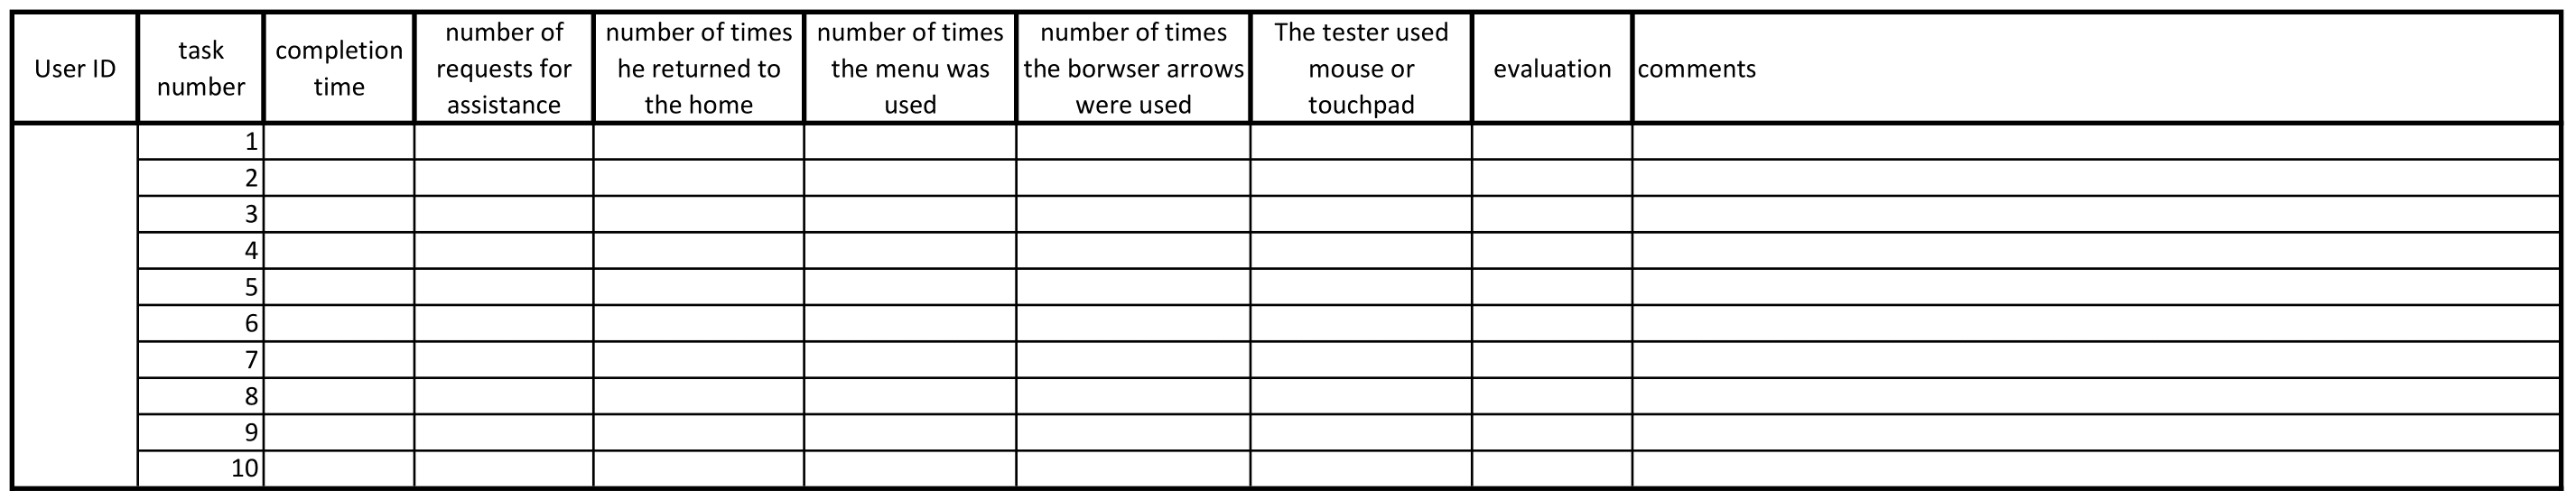
\includegraphics[width=18cm]{images/user testing/Sample_sheet.png}
        \caption{Examiners sheet structure}
        \label{fig:my_label}
    \end{figure}
\end{itemize}

\subsubsection{After Test}
Once all the tasks were completed, a final questionnaire was given to the users in order to obtain additional feedback about their opinion on the website and their personal experience. \\
It was composed of 15 different questions with closed answer (a value ranging from 1 to 5). The targeted aspects were the followings: ease and comfort of use, utility of the tools provided (e.g., menu), clarity and presentation of content. Moreover, a final textual box was given to collect any last-minute general comments about the website. \\
The questionnaire was built using as references already existing templates, such as the System Usability Scale (SUS) template, or the Questionnaire for User Interface Satisfaction (QUIS) template. \\
The answers were collected via Google Forms. \\

\subsection{Results}
\subsubsection{Effectiveness - Task success rate}
In the following diagrams we can see the score, the average score and the completion percentage obtained for each task. Here it is also provided a brief description of the tasks that collected the least and the greatest number of points. \\
\begin{figure}[H]
    \centering
    \subfigure[Completion percentage per task]{
        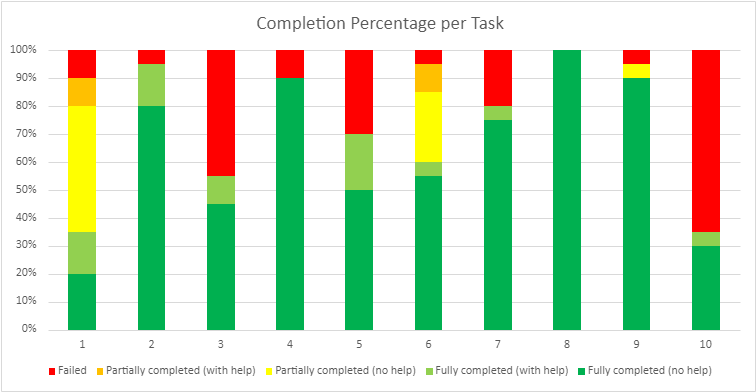
\includegraphics[width=.6\textwidth]{images/user testing/completion_percentage_per_task.png}
    }
    \subfigure[Total score per task]{
        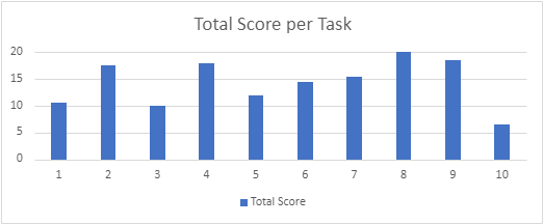
\includegraphics[width=.4\textwidth]{images/user testing/total_score_per_task.png}
    }
    \subfigure[Average score per task (with variance)]{
        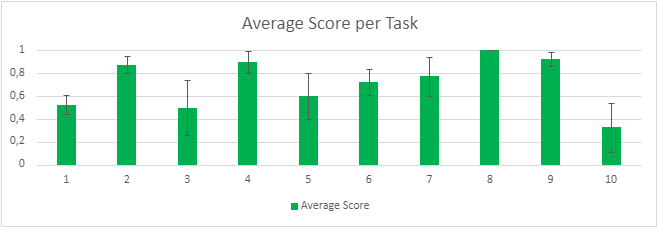
\includegraphics[width=.476\textwidth]{images/user testing/average_score_per_task_with_var.png}
    }
    \caption{Task scores and completion percentage}
    \label{fig:scores_per_task}
\end{figure}
\noindent
Least successful tasks (< 12 total points): 
\begin{itemize}
    \item \hyperref[Task:01]{Task 1} (10.5/20) $\rightarrow$ The majority of the users managed to complete the first part but had troubles in the second part (as furtherly explained in the next paragraph). 
    \item \hyperref[Task:03]{Task 3} (10/20) $\rightarrow$ The video experience was penalized enough by the fact that almost all the users reached a video, but not always the requested one (gap year student).
    \item \hyperref[Task:10]{Task 10} (6.5/20) $\rightarrow$ The majority of the users reached the Dublin page of “Music \& Performing Arts Internships” instead of the Ireland one. As supposed by the examiners (see the motivation of the task), these ambiguity and inconsistency mislead many users to the wrong result. 
\end{itemize}
Most successful tasks (>= 18 total points): 
\begin{itemize}
    \item \hyperref[Task:04]{Task 4} (18/20) $\rightarrow$ The “TIME” article was found by almost everyone, and ¾ of the users directly saw and used the blue banner, which is present in all the pages.
    \item \hyperref[Task:08]{Task 8} (20/20) $\rightarrow$ The UK telephone number was found by everyone, both at the bottom of the page and in the “Contact us” section. 
    \item \hyperref[Task:09]{Task 9} (18.5/20) $\rightarrow$ The “academic credit” page is clearly visible in the “how it works” menu. 
\end{itemize}

\subsubsection{Efficiency - Time on task}
In the following diagram we can see the average time required for each task. Here it is also reported a brief description of the task that required the lowest and greatest amount of time to complete. \\
\begin{figure}[H]
    \centering
    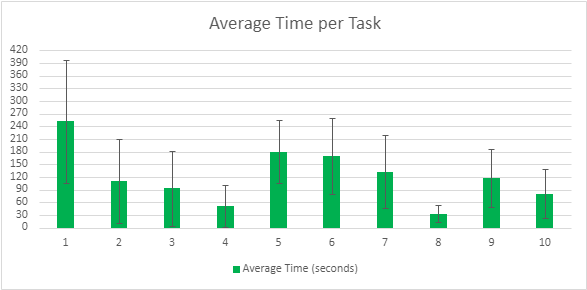
\includegraphics[width=.6\textwidth]{images/user testing/average_time_per_task_with_var.png}
    \caption{Average time per task (with standard deviation)}
    \label{fig:time_per_task}
\end{figure}
\noindent
The fastest tasks (under 1:30 min) were: 
\begin{itemize}
    \item \hyperref[Task:04]{Task 4} (0:51 min) $\rightarrow$ It was quick because the banner in the home page was easily seen by the majority of the users. 
    \item \hyperref[Task:08]{Task 8} (0:32 min) $\rightarrow$ It was very quick because the position of the telephone number followed the standard, in fact almost every user found it at the bottom of the page. 
    \item \hyperref[Task:10]{Task 10} (1:19 min) $\rightarrow$ It was very quick because the menu was easily navigable from “career fields”.
\end{itemize} 
The slowest tasks (over 2:30 min) were: 
\begin{itemize}
    \item \hyperref[Task:01]{Task 1} Task 1 (4:11 min) $\rightarrow$ It required a lot of time to complete mainly because of the second part of the task (finding the eligibility for New York), while the first part was usually completed quickly by the participants. The main observed obstacle was the term “Visa”, which was present in the left-side menu in the New York page (“Visa information for New York”) that many participants reached: almost everyone thought of it as something regarding money (as for Visa/MasterCard), so very few clicked on that specific section. It is also peculiar that all the links directly available in the “Eligibility” page are named as “Visa requirements for <destination>”, while the redirected page (and the name of that section in the left-side menu of that destination page) is named as “Visa information for <destination>”). In the end, this could be only a linguistic issue, but apparently it can in any case mislead many foreign people. 
    \item \hyperref[Task:05]{Task 5} (2:59 min) $\rightarrow$ It required much time because the “Summer Internships” page is placed in “Destinations”, while many users went searching for it in “Program fees \& Start dates”. In the end, the examiners suspect of the misplacement of the “By Season” voice (as explained in the motivation of the task) was confirmed by the behaviour of the users. 
    \item \hyperref[Task:06]{Task 6} (2:49 min) $\rightarrow$ It required quite some time because people had troubles in finding the blog, which is only reachable from a small button at the bottom of the page. The newsletter subscription form, instead, was found pretty quickly. 
\end{itemize}

\subsubsection{Usage of navigation elements}
In the following diagrams we can see the average number of times the users have used the following navigation tools: Home shortcut, browser arrow and upper menu. Here it is also given a short explanation of the results these data may infer. \\
\begin{figure}[H]
    \centering
    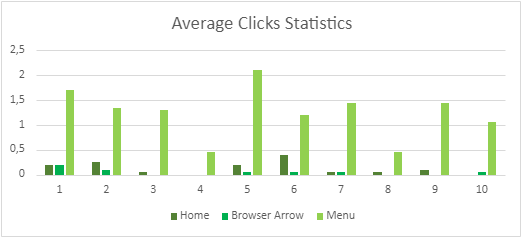
\includegraphics[width=.6\textwidth]{images/user testing/average_clicks_statistics.png}
    \caption{Average number of clicks}
    \label{fig:clicks_stats}
\end{figure}
Navigation tools: 
\begin{itemize}
    \item Home $\rightarrow$ The Home shortcut has rarely been used, since the home page doesn’t provide any particular additional link with respect to the other pages. 
    \item Browser Arrow $\rightarrow$ The users, having received the indication of using the browser arrow as little as possible, managed to give priority to the available links in the page, resulting in a low usage of this navigation tool. The only cases in which it has been used are mainly to exit the “Apply Now” page, which doesn’t present any upper menu, but only the logo (still, not so visible for some users). 
    \item Menu $\rightarrow$ The upper menu proved to be the main navigation tool used by the users. Given the fact that it is always available (apart from a few exceptions), it allows to reach very quickly any section of the website in any moment. 
\end{itemize}

\subsubsection{Comments}
This is a list of the most relevant comments that have been gathered through the questionnaire: 
\begin{itemize}
    \item \textit{The left side menu is unclear to use and browse (maybe because of the screen size). Unclear what “subscribe” in the end of the page refers to, leading uncertainty to what and where the newsletter is (problem with subscribe and blog at the end). }
    \item \textit{CONS: A lot of information, the page is too much full. Sometimes i got deviated and end up in pages that i didn't want to go to. \\
    PRO: career fields are clear and do exactly what they're supposed to. } 
    \item \textit{Lateral menu not fully visible; "Music Internships" not in alphabetical order in the career fields; Dublin and Ireland mistake/ambiguity. }
    \item \textit{The menu was user friendly although I ignored the section "who you are" due to the fact that it was too near to "who we are". However, I got more information than I had though. }
    \item \textit{The website it's quite clear. Maybe you can improve it by putting a search bar. }
    \item \textit{I would avoid putting some info only on the bottom of the page, as the blog: you keep them always visible (for instance on the side of the page) or you put them in the menu or something like that. }
\end{itemize} 
 
\subsubsection{Satisfaction}
The results of the questionnaire, which was submitted to the users after completing all the tasks, can be seen in the following diagram:
\begin{figure}[H]
    \centering
    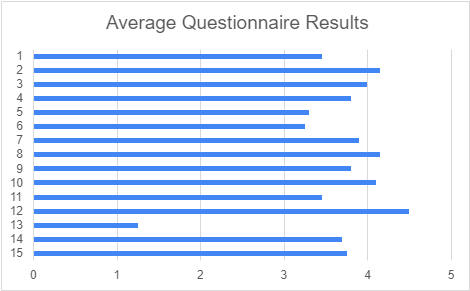
\includegraphics[width=.6\textwidth]{images/user testing/average_questionnaire_results.png}
    \caption{Average questionnaire results}
    \label{fig:question_results}
\end{figure}
\noindent
From this, we can clearly see that the majority of the scores are placed in the 3 to 4 range. This means that the overall opinion of the users about the website is sufficiently good, but there is still room for improvement. After all, the very first question (\#1) is about the general description of the website and its score is 3.45/5. \\
More specifically, the higher scores (> 4 points) are related to the aesthetics and visual design (\#2) and readability (\#12) of the website, while also to the clearness of input prompts (\#8) and the usefulness of the menu (\#10). \\
The lowest score (\#13), instead, is not problematic since it expresses the amount of errors the users found on the website, which was very low. In fact, no user found errors like the “404 not found” one, which was instead seen during the inspection. \\
The lowest scores among the other questions, however, express some criticism against the difficulty level of finding the requested information on the website (\#5) and the expected time to perform such action (\#6). Moreover, also the easiness of scrolling the pages (\#11) stands out as one of the least appreciated parts of the website. \\
\\
In the end, through this questionnaire, the most problematic elements which have been perceived by the users are mainly related to navigation, while content and presentation aspects are reasonably ok. The only navigation element that positively stands out is the menu, which confirms itself again as the main useful navigation tool provided, even though it could be improved. 

\section{Conclusions}
\begin{enumerate}
    \item[o] Error Page
        \begin{itemize}
            \item Problem: The error page contains the error code, and it doesn't explain the problem. Indeed, it doesn’t have a turn back button, but the user is obliged to go back to the homepage.
            \item Solution: Add a clearer message about the problem that causes the error, add a back button to go back to the last page visited.
        \end{itemize}
    \item[o] Too long pages
        \begin{itemize}
            \item Problem: Some pages are too long (e.g., Homepage, "Who you are" subpages, some career field pages, etc) and it is annoying to scroll them.
            \item Solution: Split these too long pages into more pages that are navigable through a left side submenu, as it happens in destination pages (see image of inspection).
        \end{itemize}
    \item[o] Repetitive content
        \begin{itemize}
            \item Problem: A lot of pages contain repetitive contents (e.g., The Our program paragraph, the Join our global alumni network paragraph etc.). These contents use a lot of space, and they aren’t needed.
            \item Solution: remove them from the pages when not needed (all pages except for the homepage).
        \end{itemize}
    \item[o] Hidden Blog
        \begin{itemize}
            \item Problem: The Blog page is difficult to find, since it is only reachable by a small button at the bottom of the page. In fact, many users overlooked that link.
            \item Solution: Add a link to the Blog from the “Who we are” menu, in the same way as it is for the “In the media” page (upper menu + bottom page links), in order to be more easily reachable. 
        \end{itemize}
    \item[o] "Apply Now" Page
        \begin{itemize}
            \item Problem: The “Apply Now” page is some sort of point of no return for the user’s navigation. Especially when accidentally opened, the lack of any information status and of the upper menu often puzzled the user, which struggled to go back. Moreover, the page would sometimes open in a new tab, sometimes open in the same page, depending on which button is used, but their layout is always the same.
            \item Solution: Improve the navigation status visibility of the page, by adding an upper menu and/or some back buttons. Furthermore, uniform the “Apply Now” buttons’ behaviour throughout the website: always open the page in a new tab, or always in the same tab, in order to remove this inconsistency.
        \end{itemize}
    \item[o] Adding a search bar for destination and career field filtering
        \begin{itemize}
            \item Problem: In order to search a specific internship in a career filed, the user has to go through the destination or career field page. This way to find these information is cumbersome.
            \item Solution: Create a search bar based on two main filters: destinations and career field. This filter can be opened as a drop-down menu after clicking on an icon in the main menu. This component can help the user searching for the information he is interested in.
        \end{itemize}
    \item[o] Inconsistency between cities and Countries.
        \begin{itemize}
            \item Problem: On the website there are inconsistencies between some cities that are available for an internship while their relative country is not shown in the "destinations" menu (e.g. There's an available internship for IT in Italy but is not shown as a destination).
            Furthermore for some internships is shown both the country and a city where you can take part into an internship (e.g. for Music internship there are both Ireland and Dublin shown in the same page).
            \item Solution: If a city is available for an internship, show its country inside Destination. Group internships available in a specific city together with those available for the same country.
        \end{itemize}
     \item[o] "Who we are" drop menu is not clear.
        \begin{itemize}
            \item Problem: Confusing naming and Inconsistencies between sub-menu entries.
            \item Solution: Naming the Menu item "About us", the sub menu has unnecessary entries that could be merged into one. 
            The left navigation menu of this voice is different from all the other in the website. While in other pages it lets the user navigate among different pages within the same topic, here the navigation remains within the entries of the menu.
        \end{itemize}
\end{enumerate}   

\newpage


\section{Annex}
\subsection{Inspection}
    \begin{figure}[H]
        \centering
        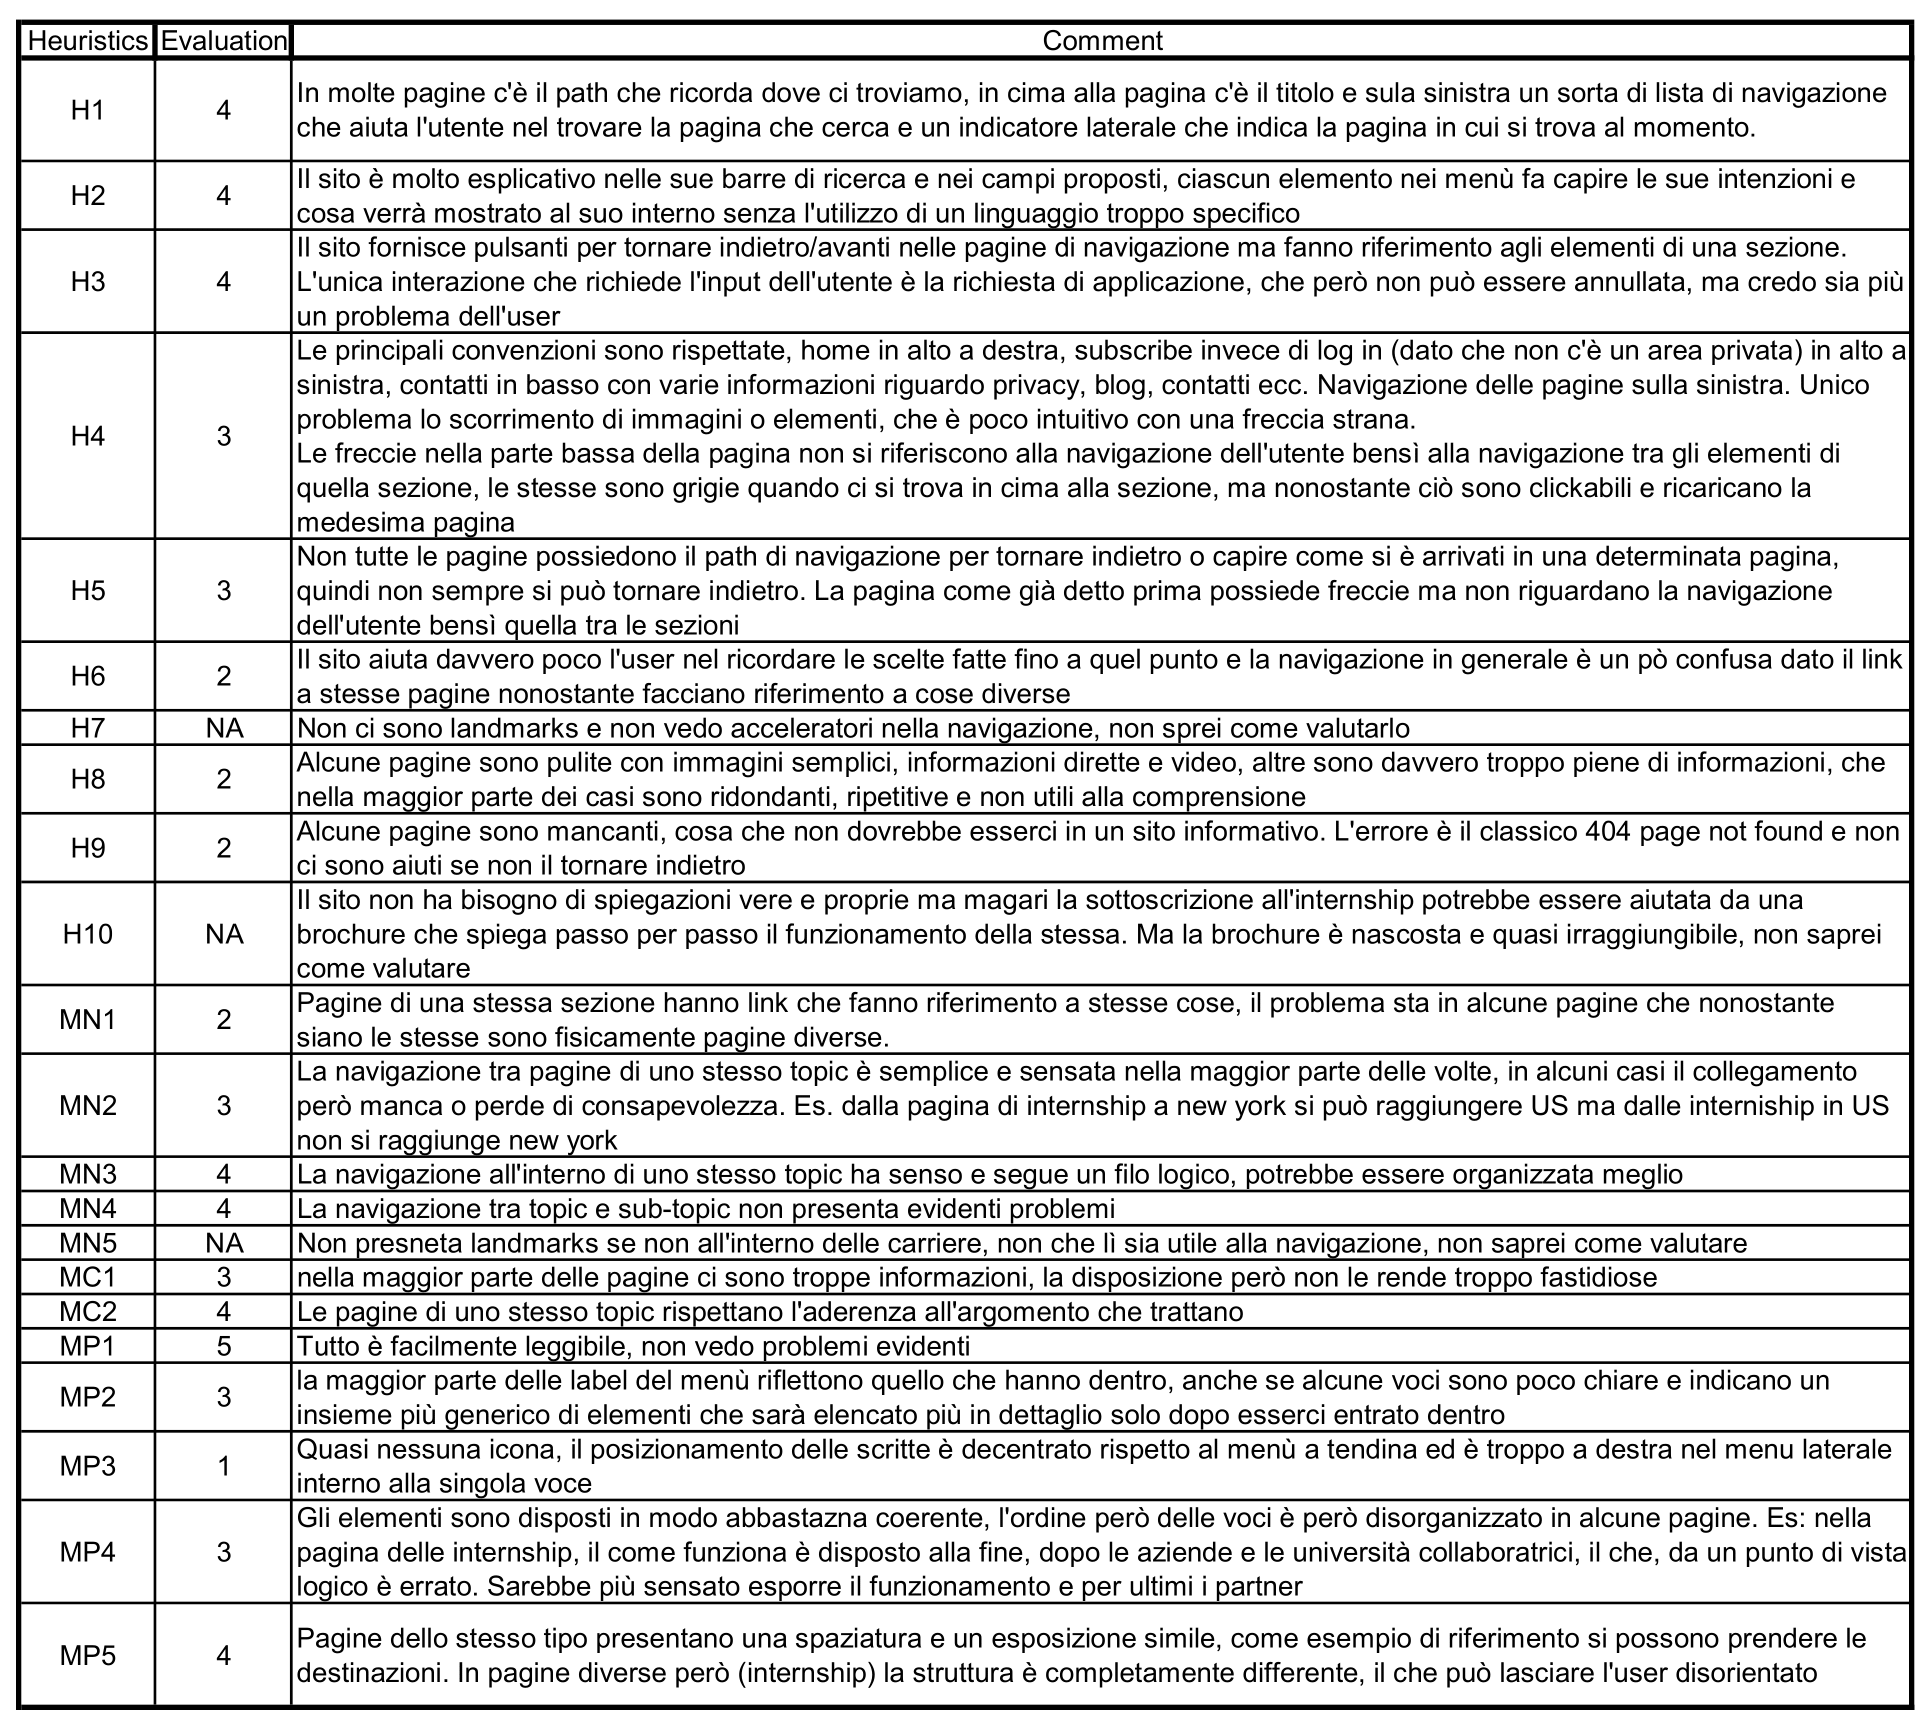
\includegraphics[width=18cm]{images/annex/DD_inspection.png}
        \caption{Inspection sheet of Davide Di Marco}
    \end{figure}
    \begin{figure}[H]
        \centering
        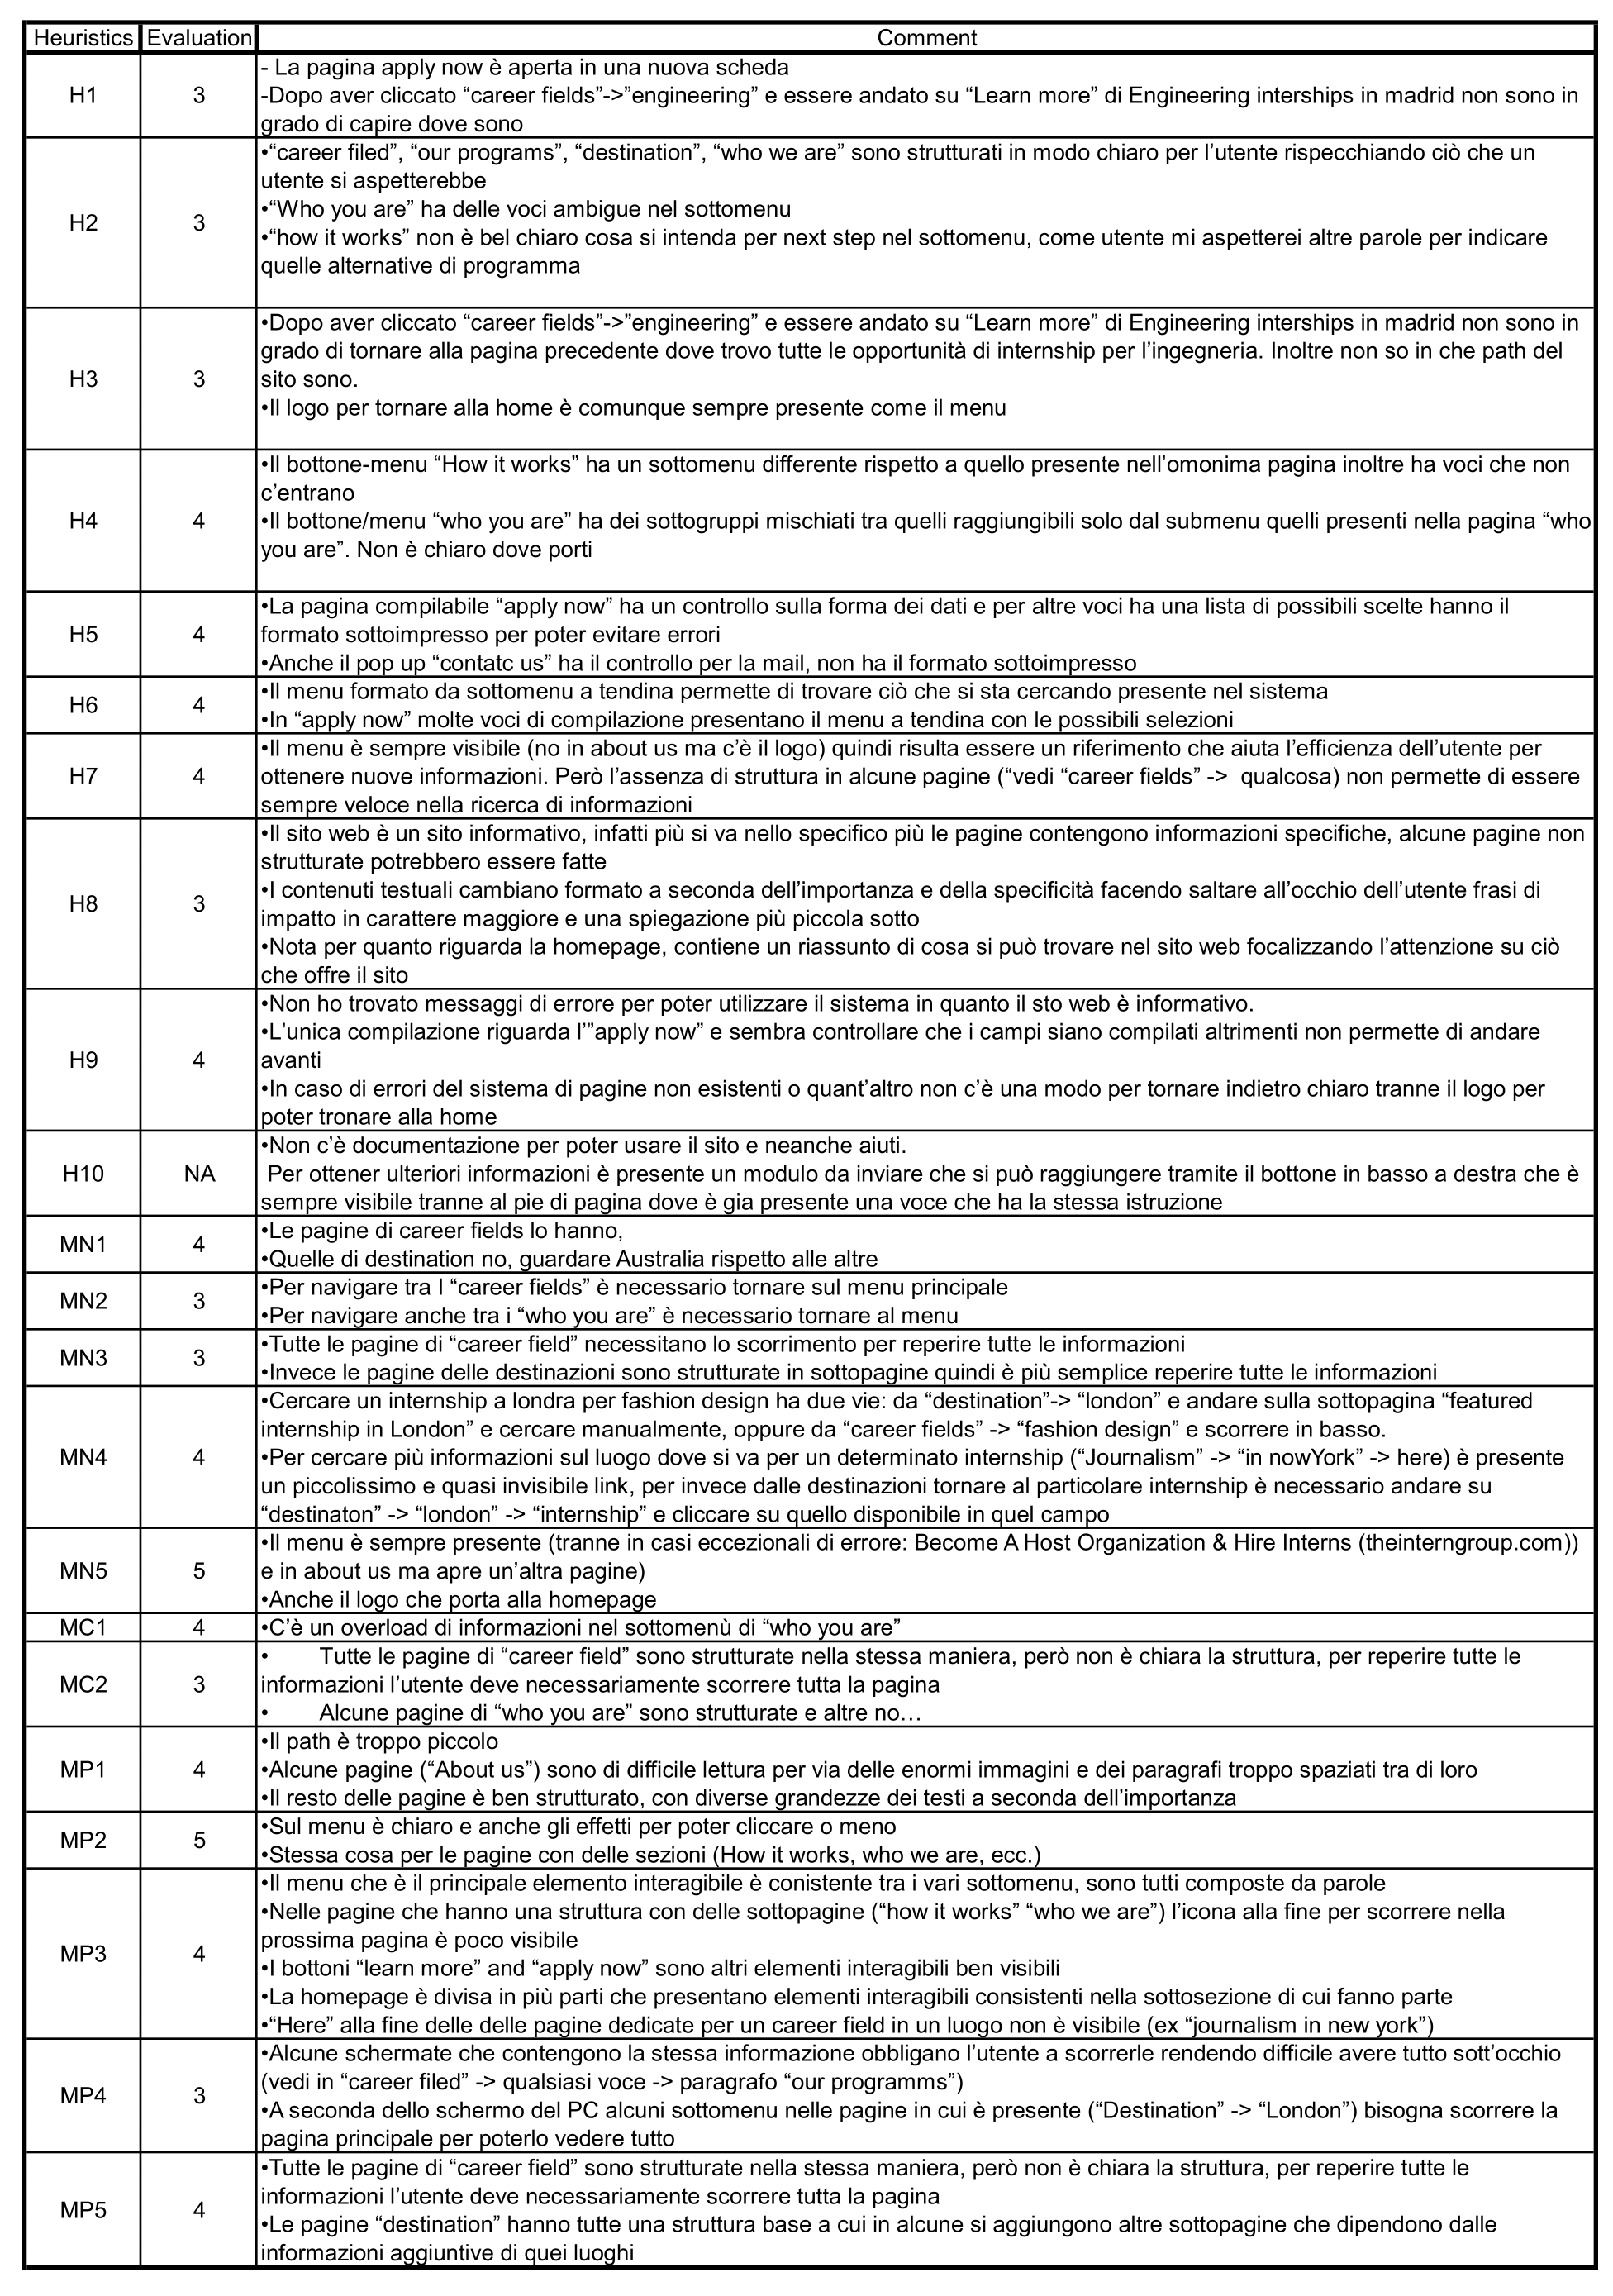
\includegraphics[width=18cm]{images/annex/SF_inspection.png}
        \caption{Inspection sheet of Stefano Fossati}
    \end{figure}
    \begin{figure}[H]
        \centering
        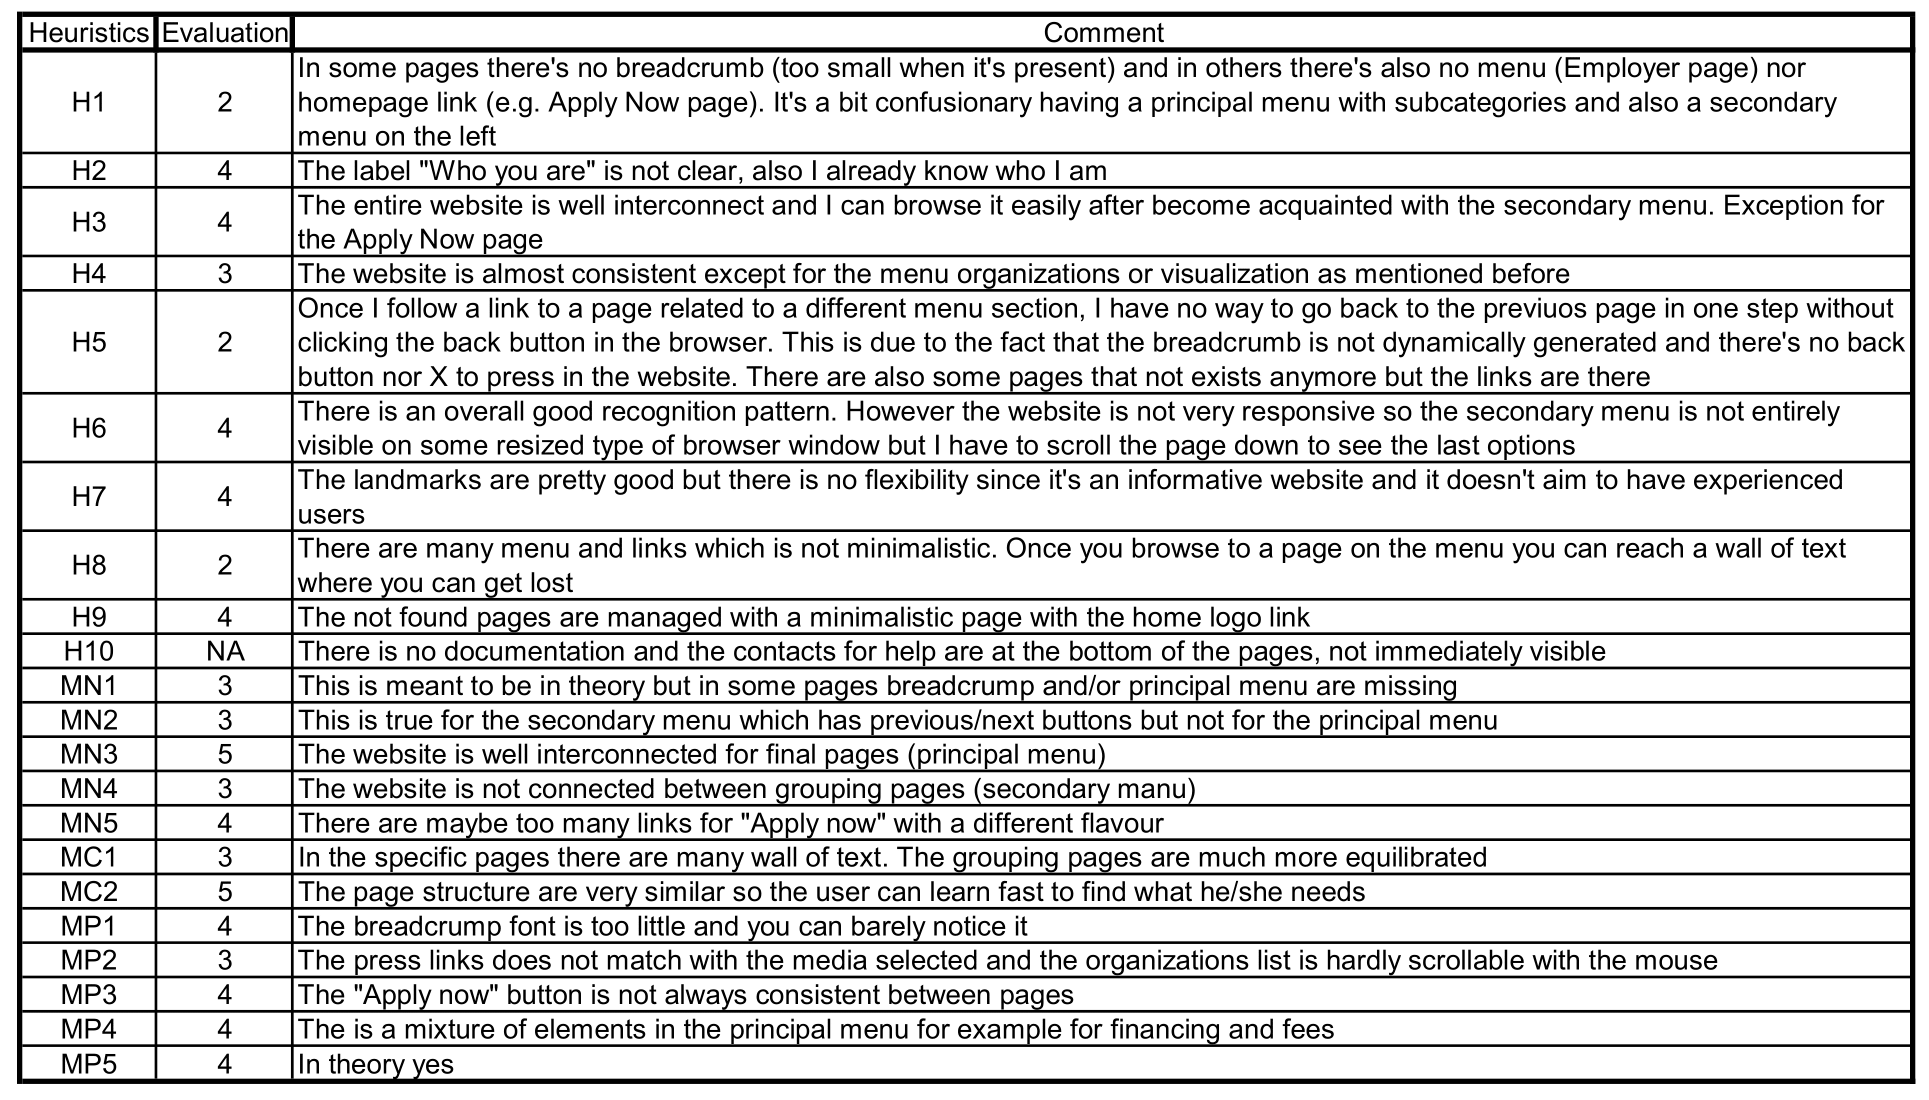
\includegraphics[width=18cm]{images/annex/DM_inspection.png}
        \caption{Inspection sheet of Davide Maffi}
    \end{figure}
    \begin{figure}[H]
        \centering
        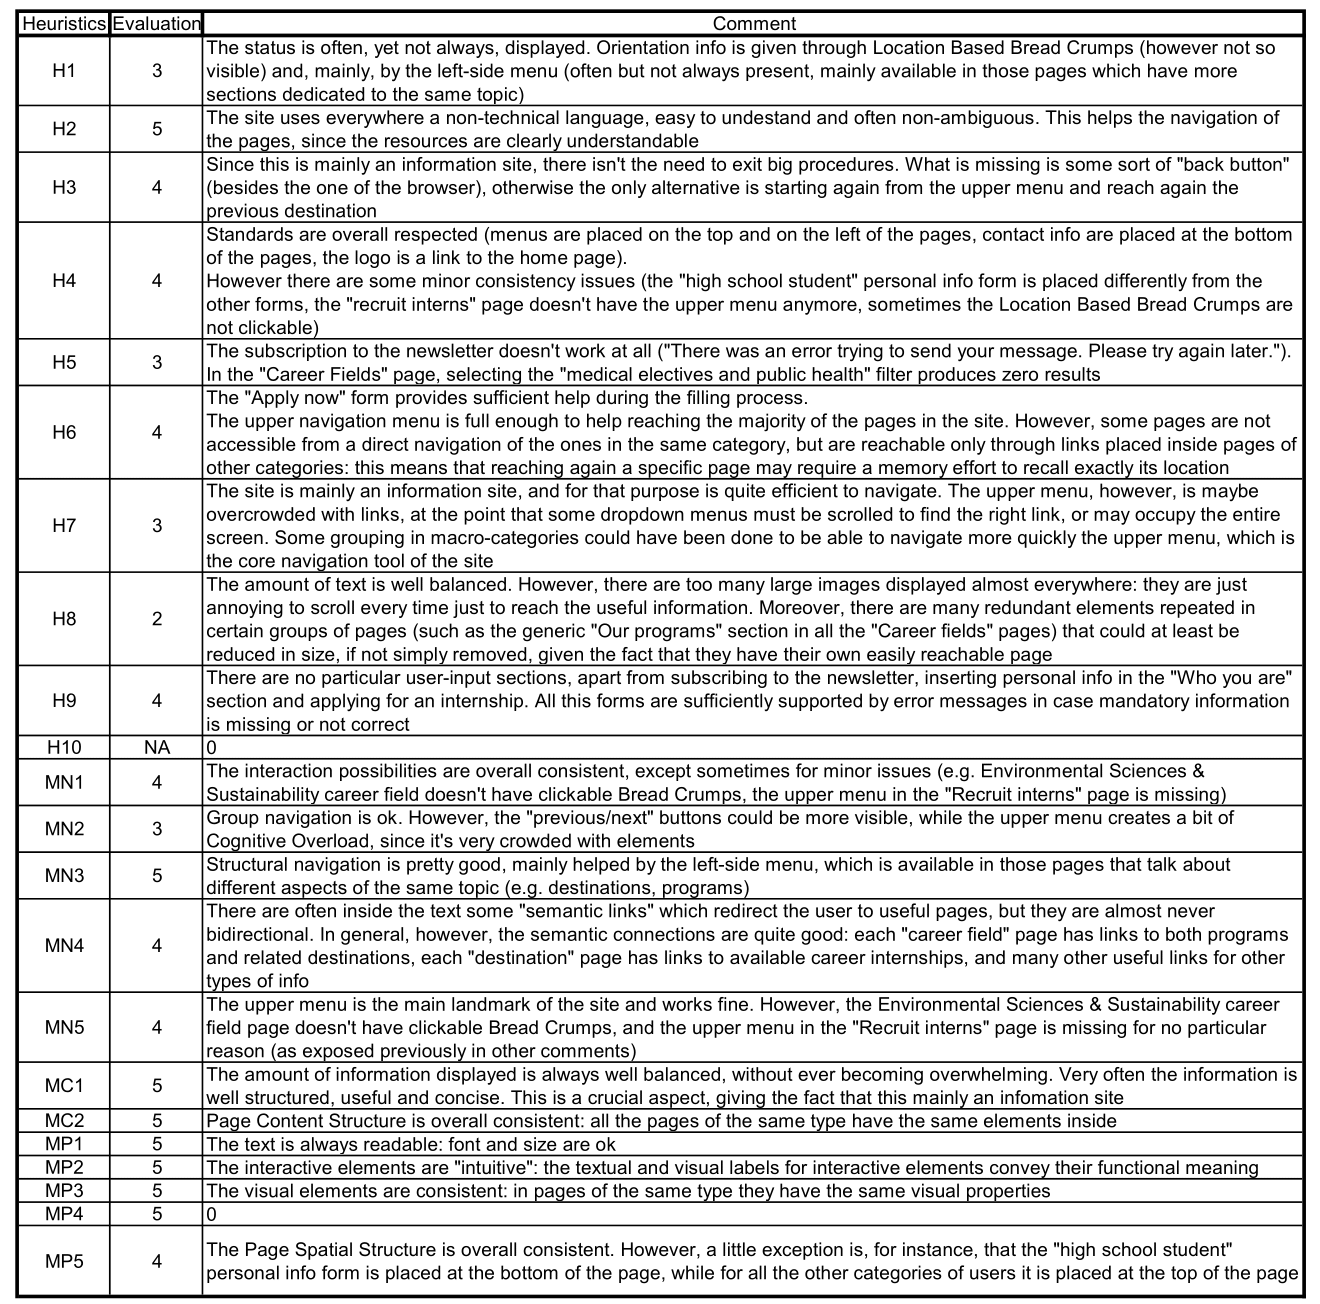
\includegraphics[width=18cm]{images/annex/MR_inspection.png}
        \caption{Inspection sheet of Marco Romanini}
    \end{figure}

\subsection{User Testing}
    \begin{figure}[H]
        \centering
        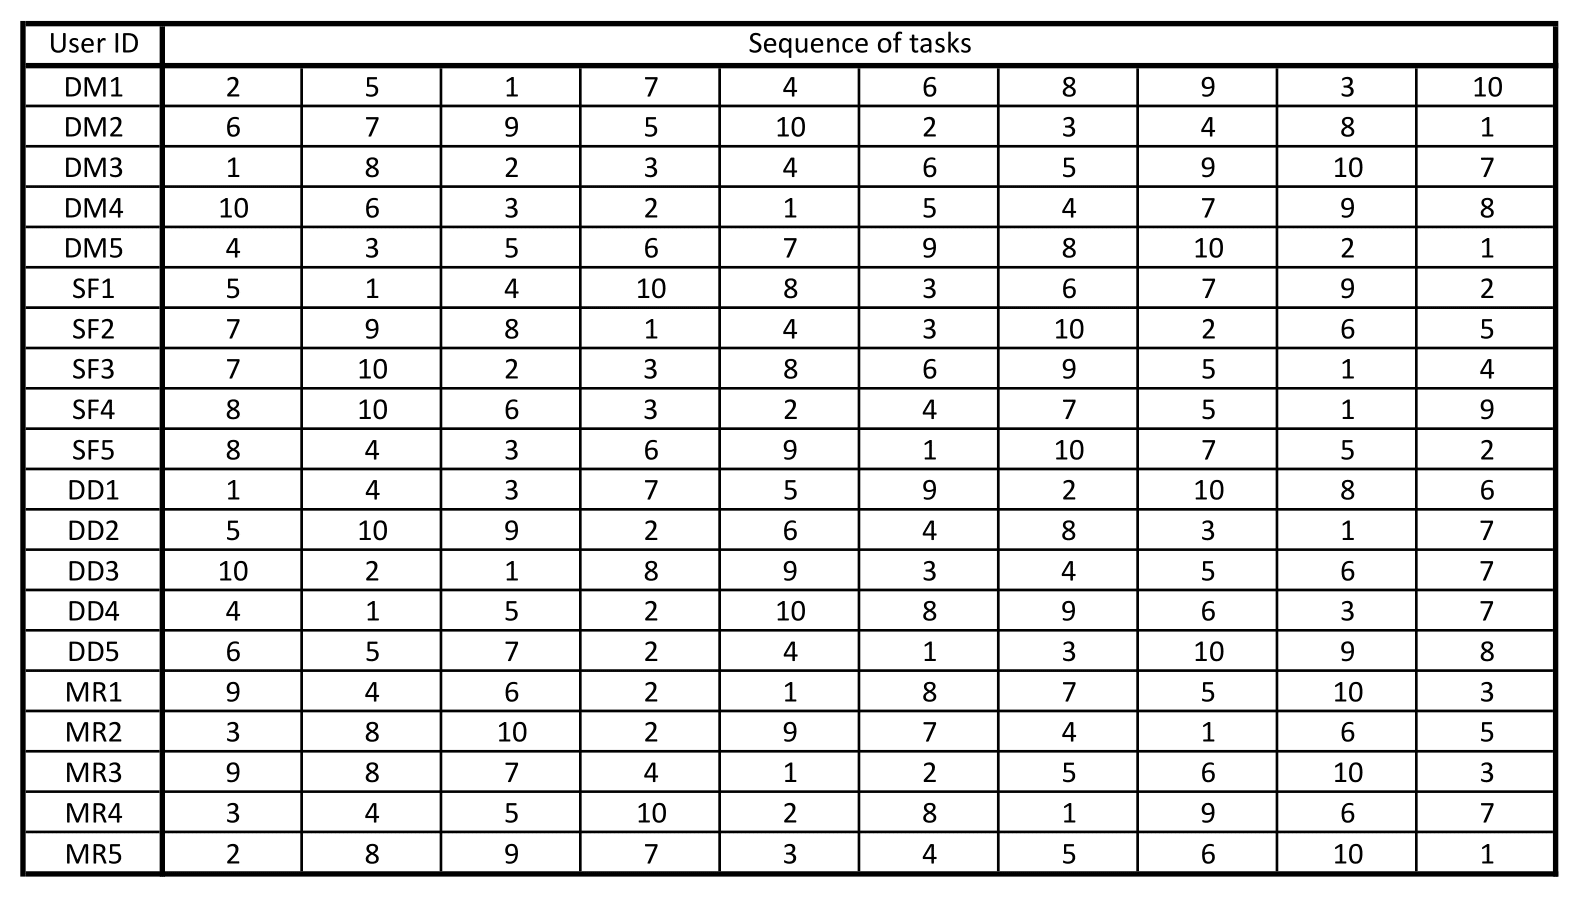
\includegraphics[width=18cm]{images/annex/Task_sequence.png}
        \label{annex:task_sequence}
        \caption{Task sequence}
    \end{figure}
    \begin{figure}[H]
        \centering
        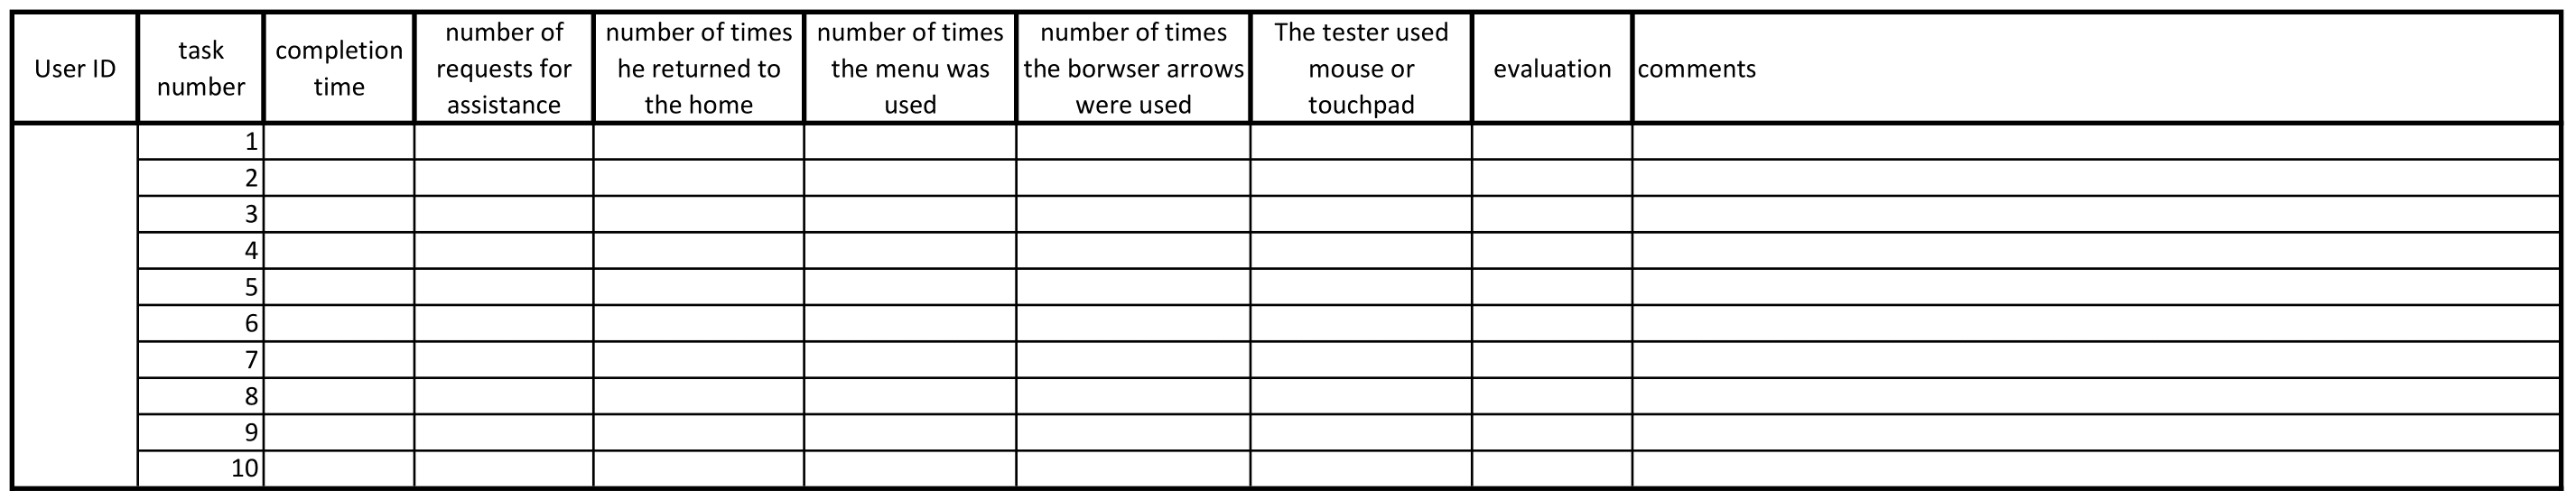
\includegraphics[width=18cm]{images/user testing/Sample_sheet.png}
        \caption{Examiners sample sheet}
    \end{figure}
\subsubsection{User testing task results}
    \begin{figure}[H]
        \centering
        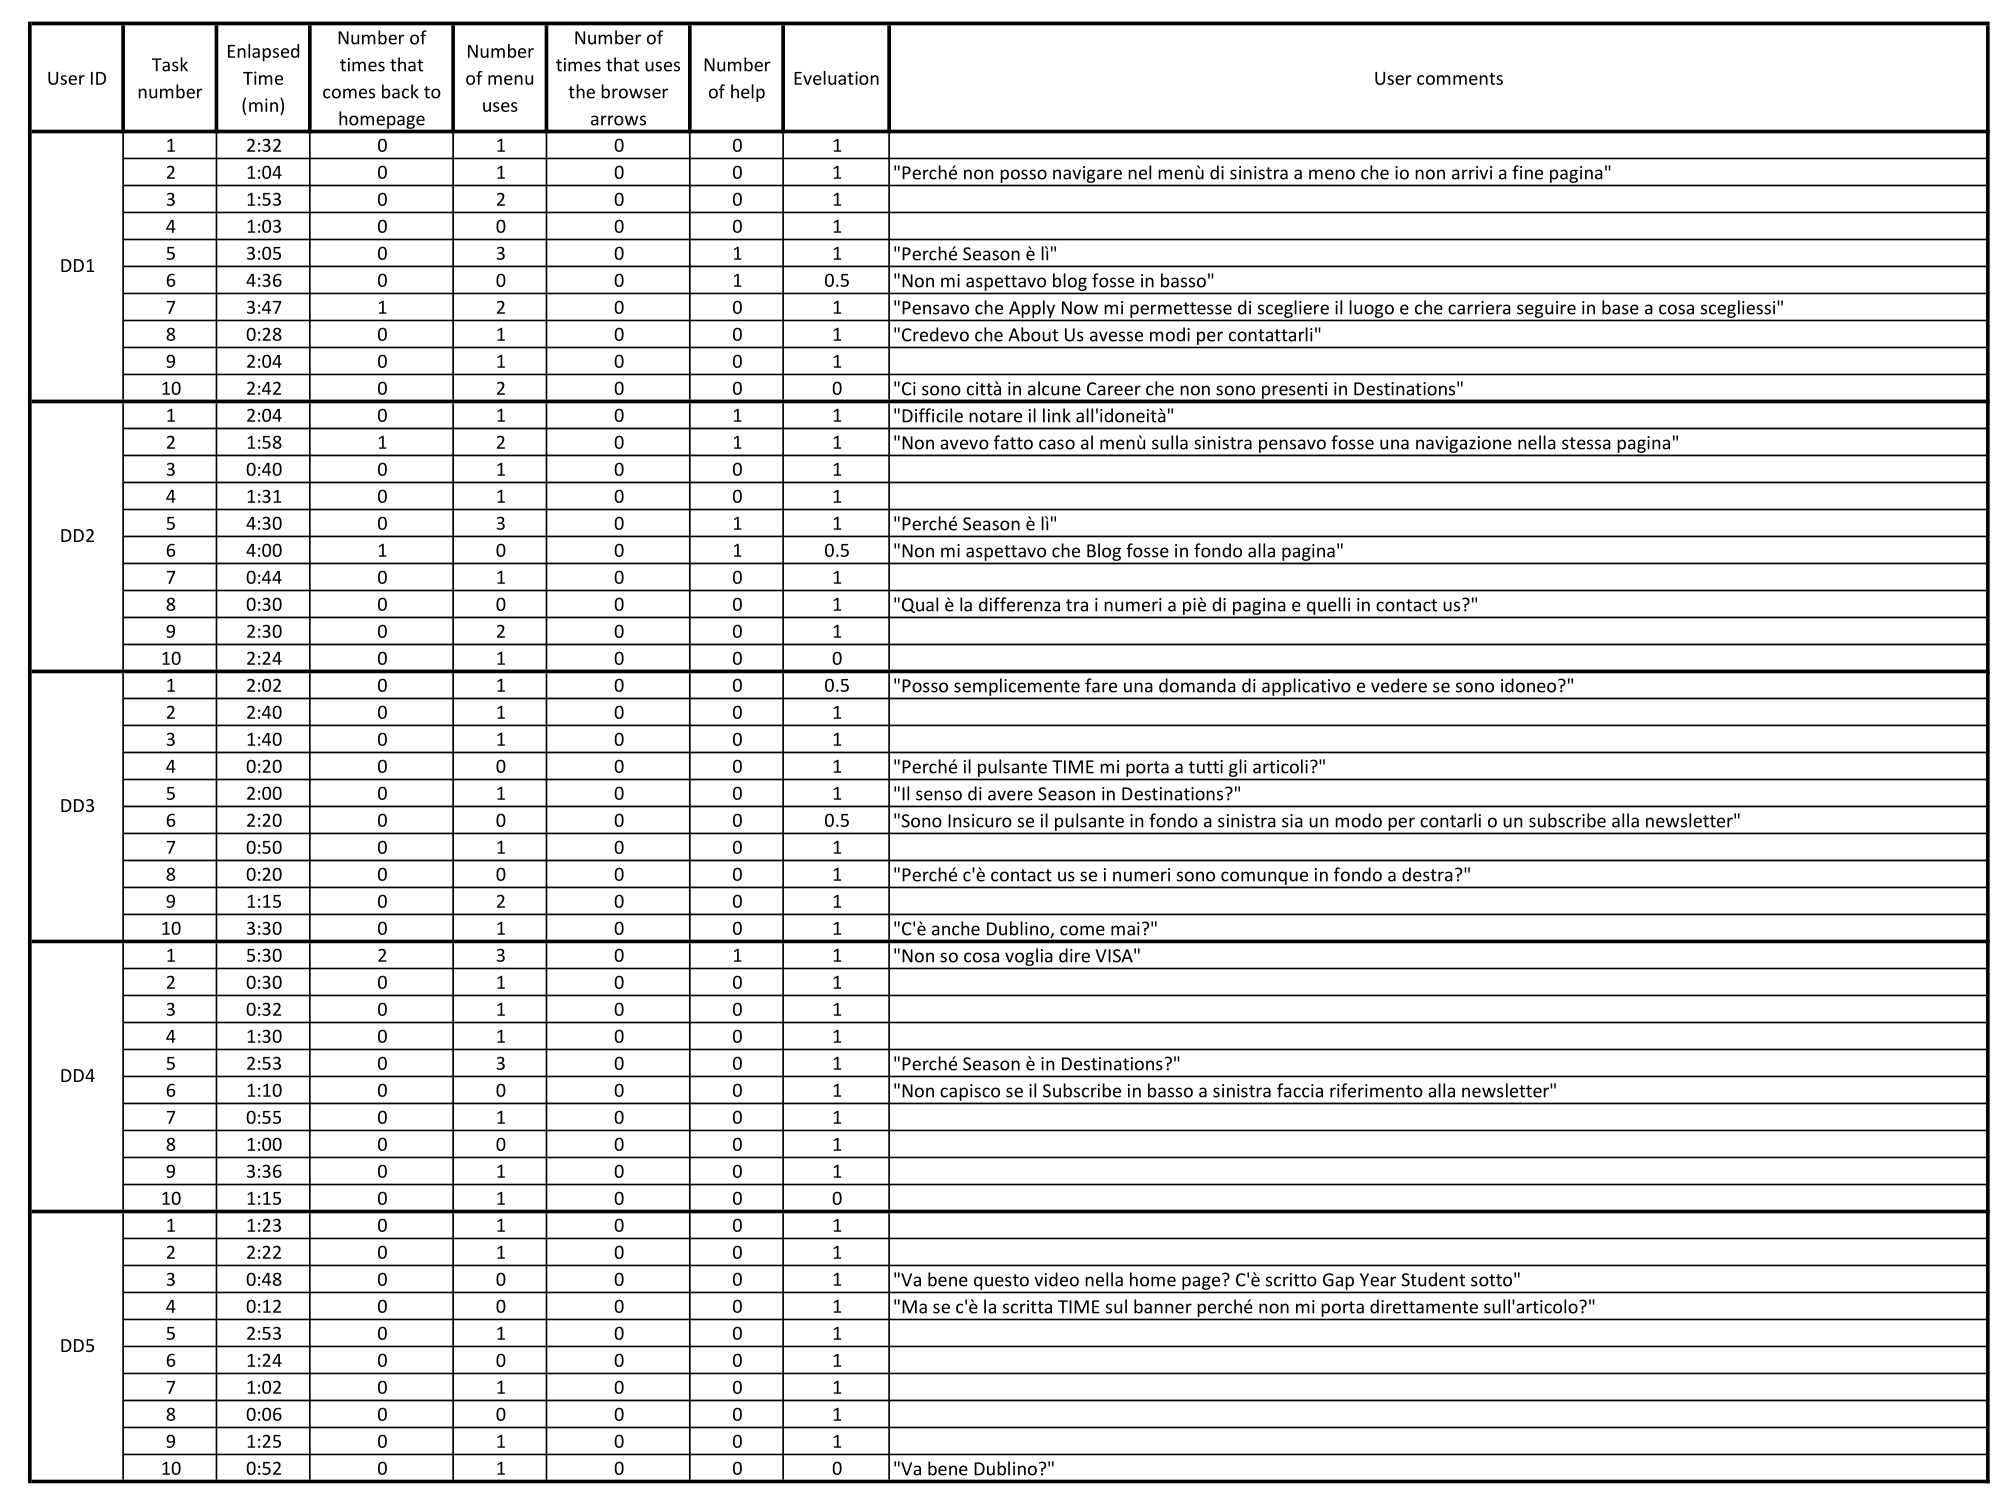
\includegraphics[width=18cm]{images/annex/DD_usertesting.png}
        \caption{Users supervised by Davide Di Marco}
    \end{figure}
    \begin{figure}[H]
        \centering
        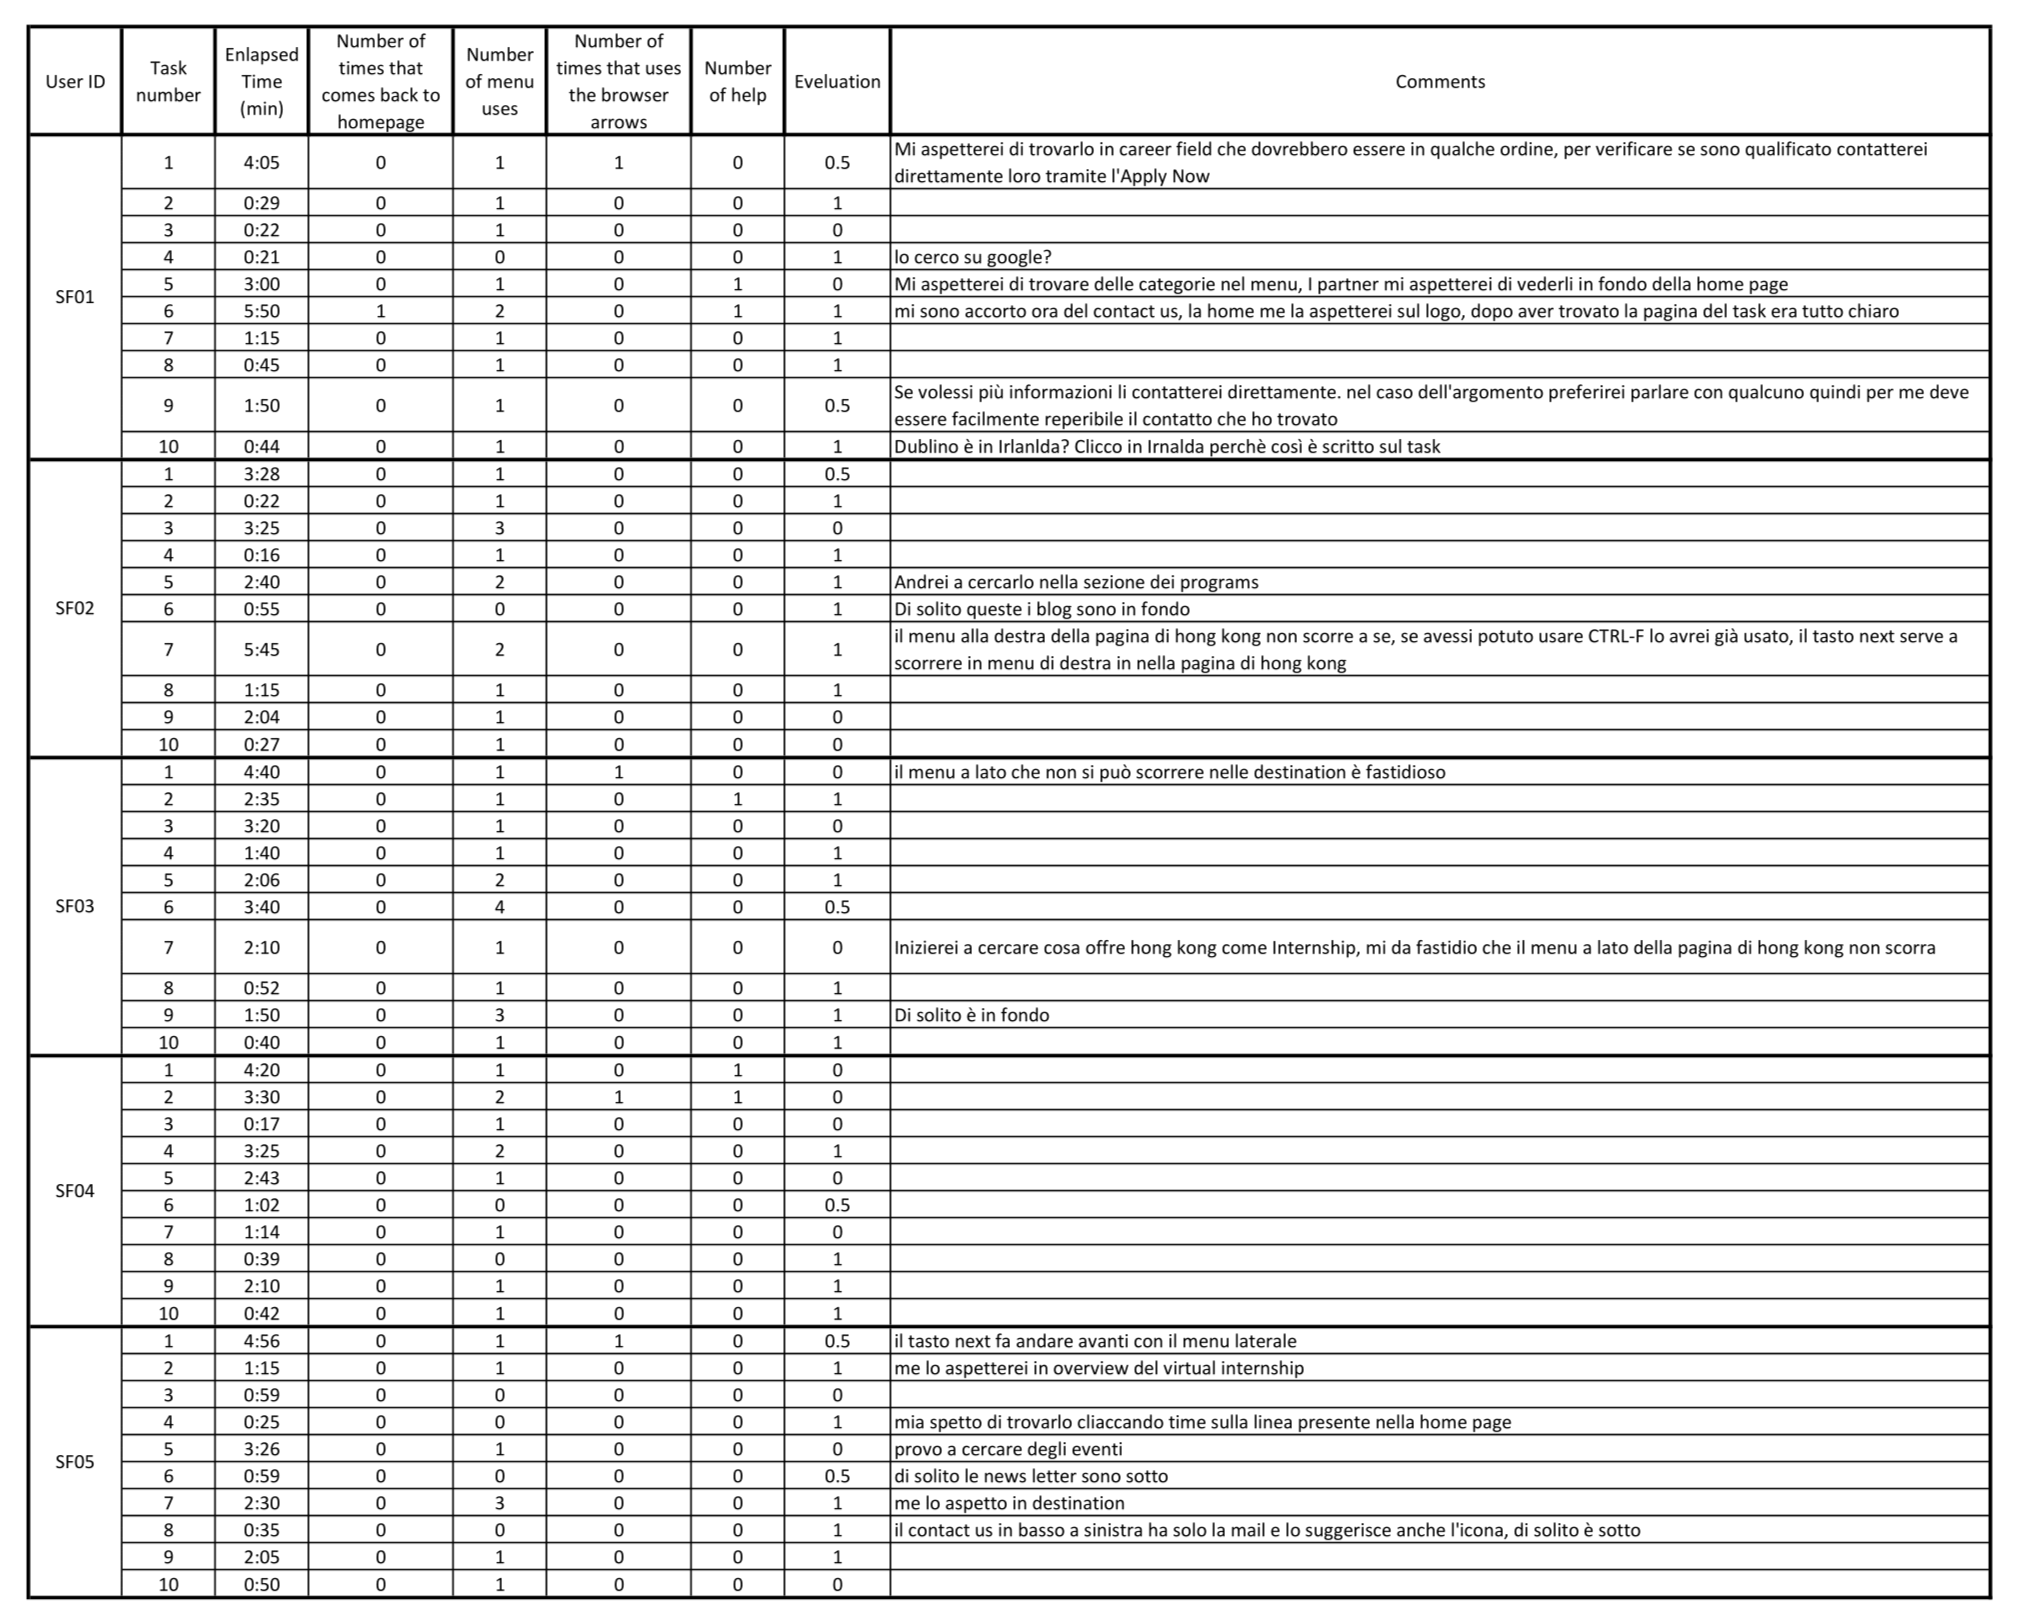
\includegraphics[width=18cm]{images/annex/SF_usertesting.png}
        \caption{Users supervised by Stefano Fossati}
    \end{figure}
    \begin{figure}[H]
        \centering
        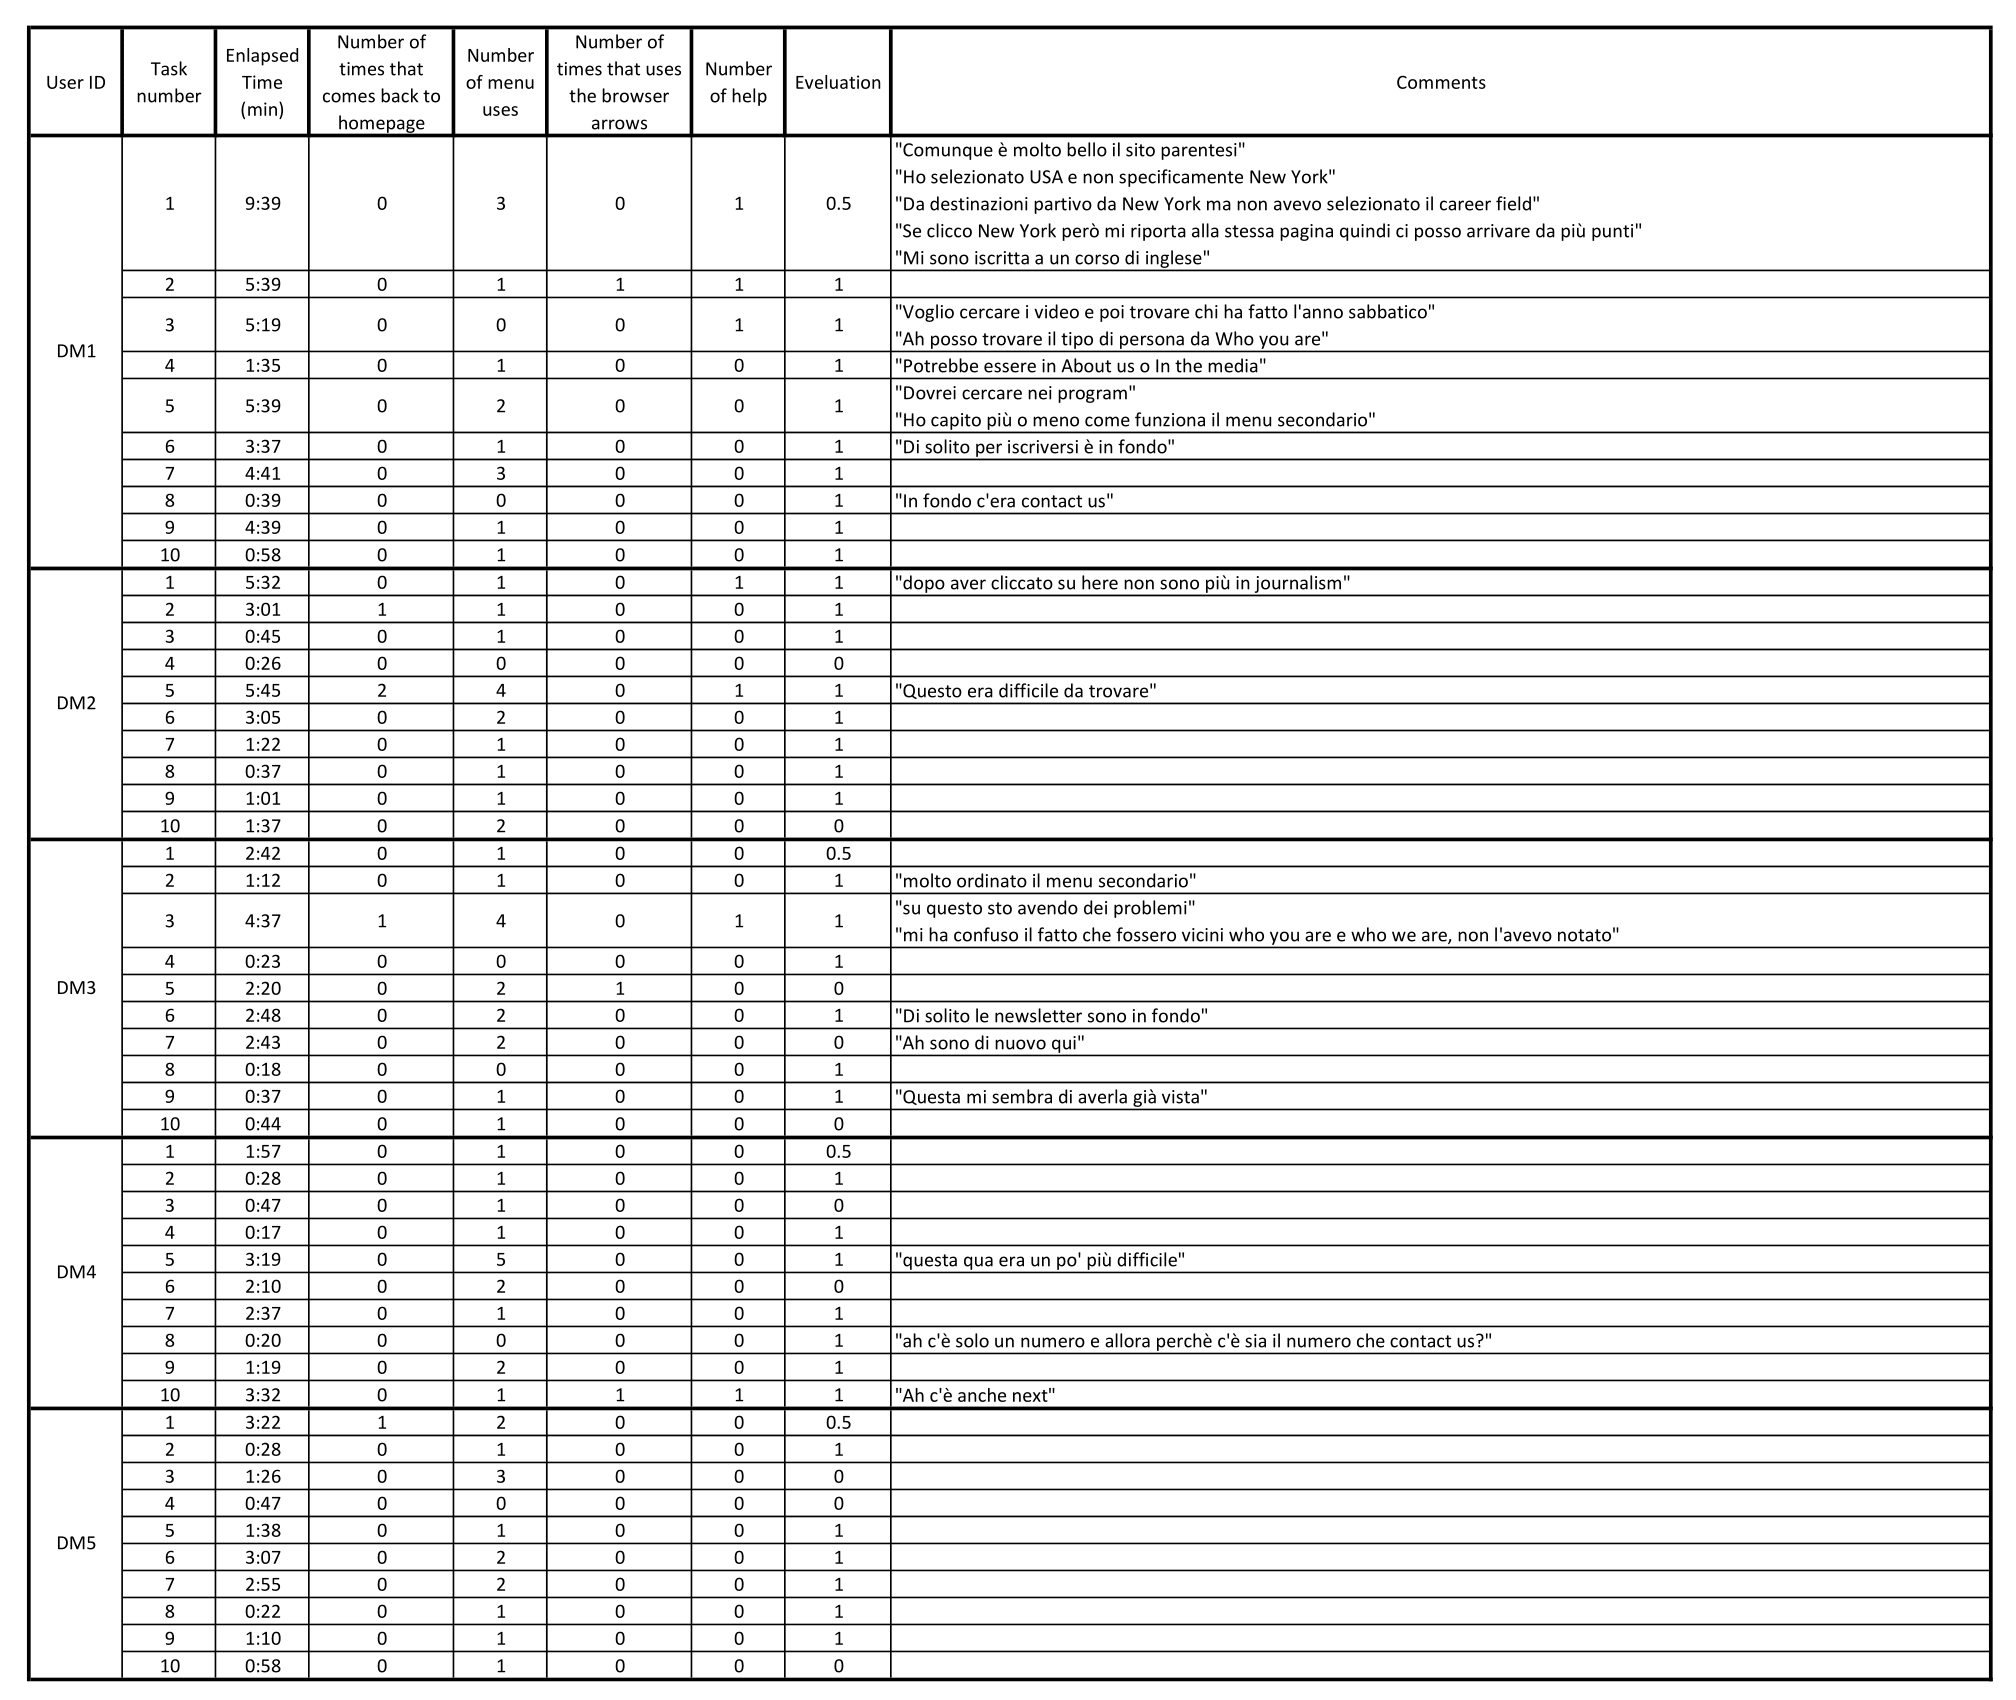
\includegraphics[width=18cm]{images/annex/DM_usertesting.png}
        \caption{Users supervised by Davide Maffi}
    \end{figure}
    \begin{figure}[H]
        \centering
        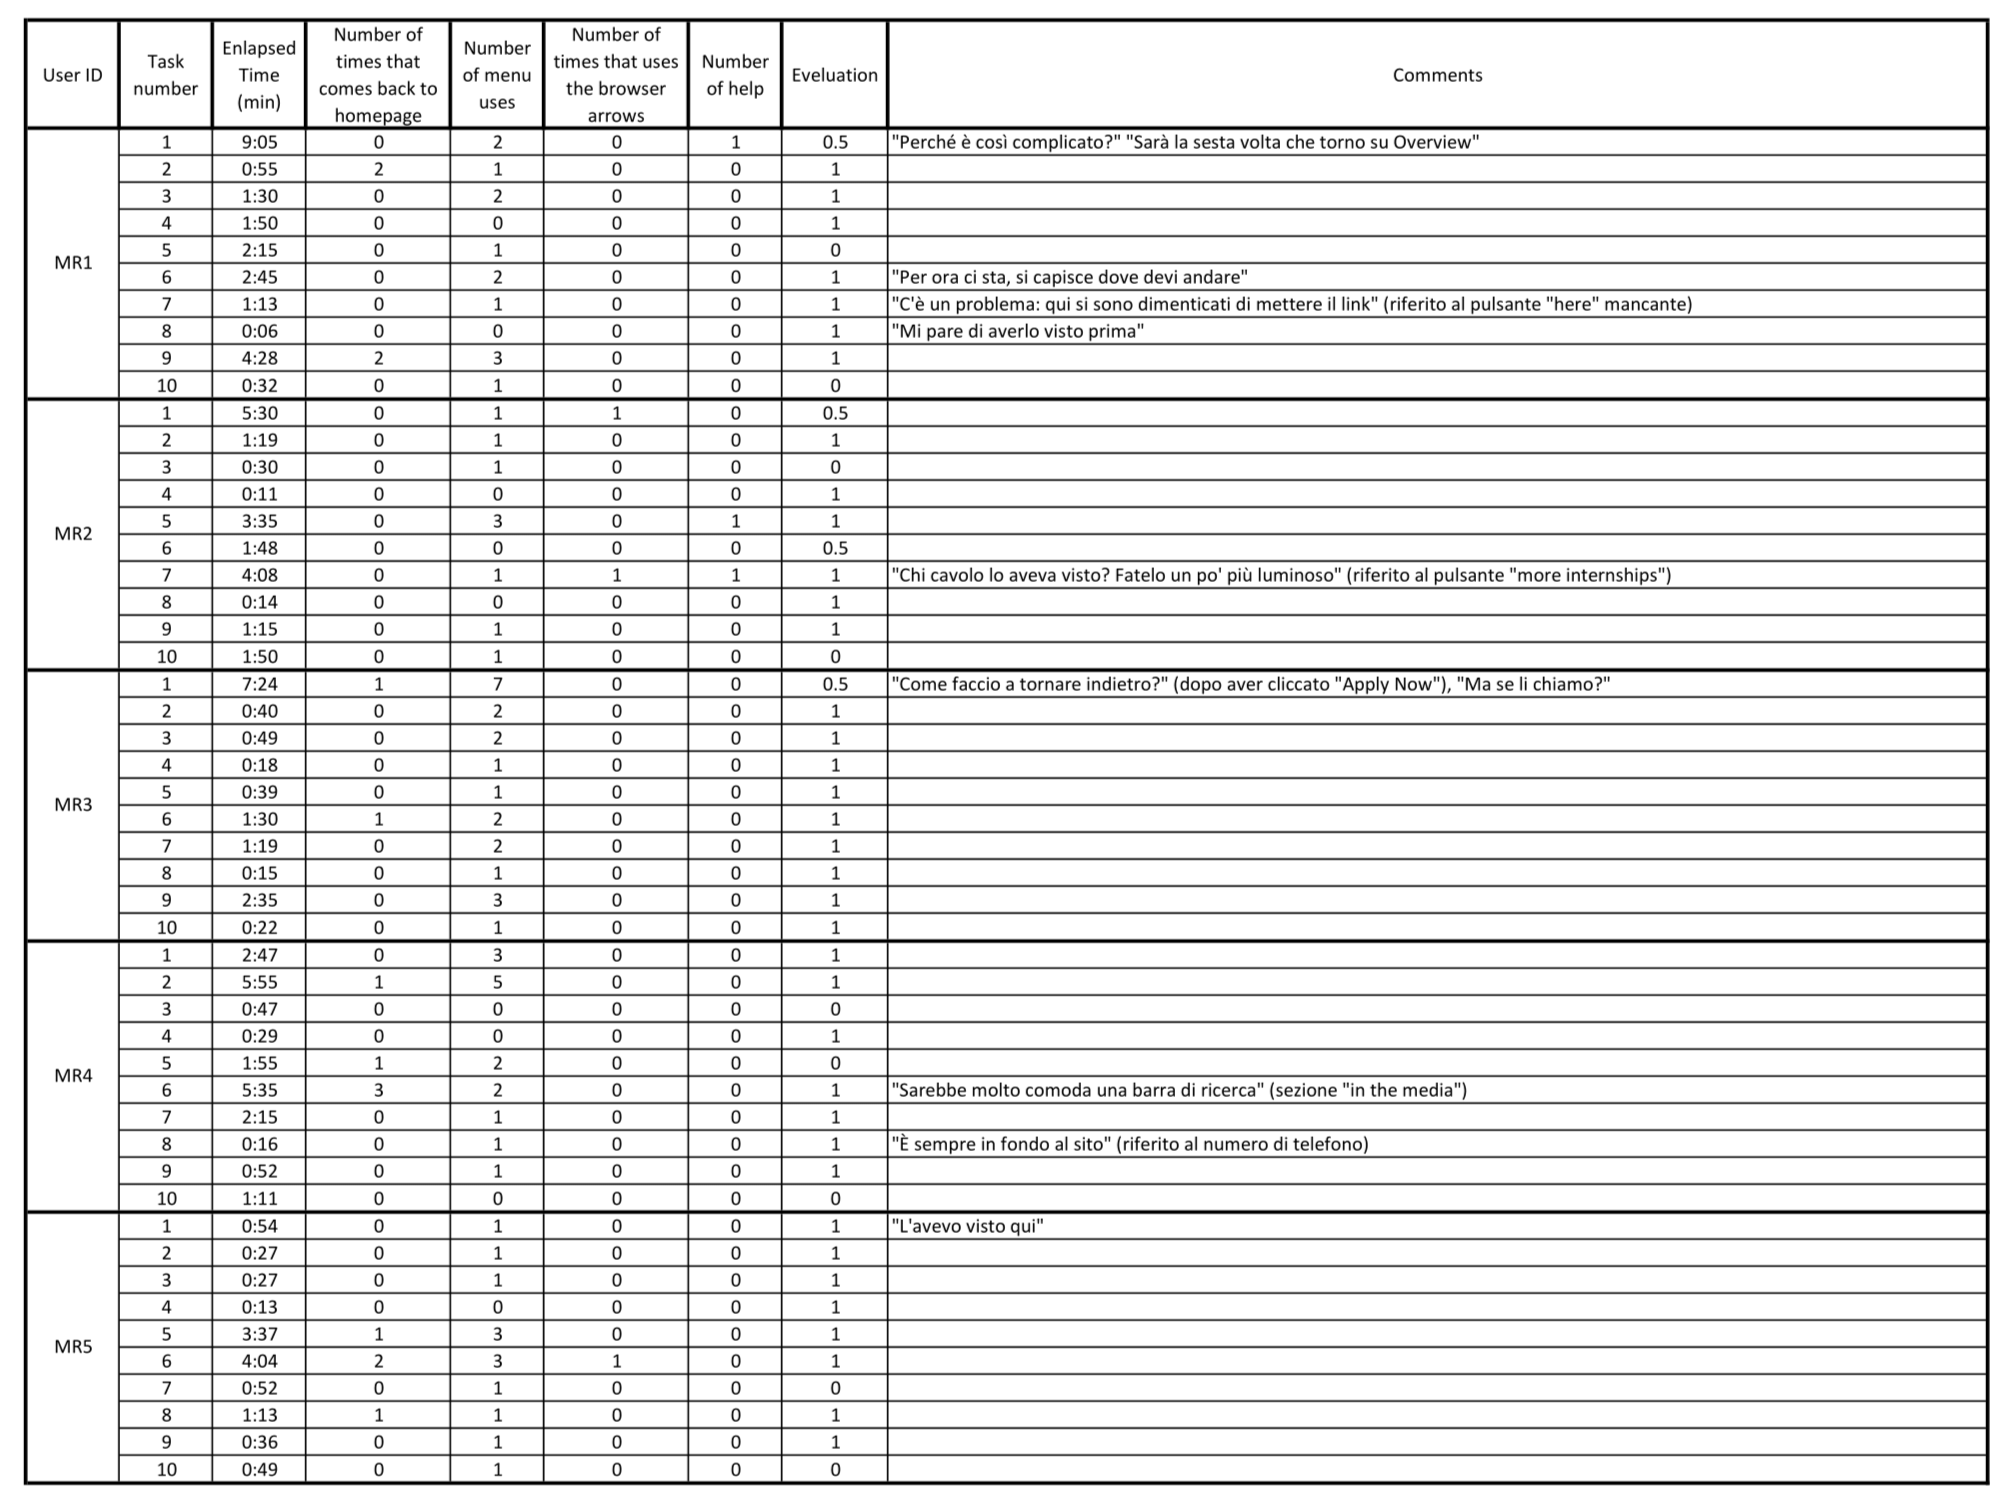
\includegraphics[width=18cm]{images/annex/MR_usertesting.png}
        \caption{Users supervised by Marco Romanini}
    \end{figure}
\subsubsection{User testing questionnaire results}
    \begin{figure}[H]
        \centering
        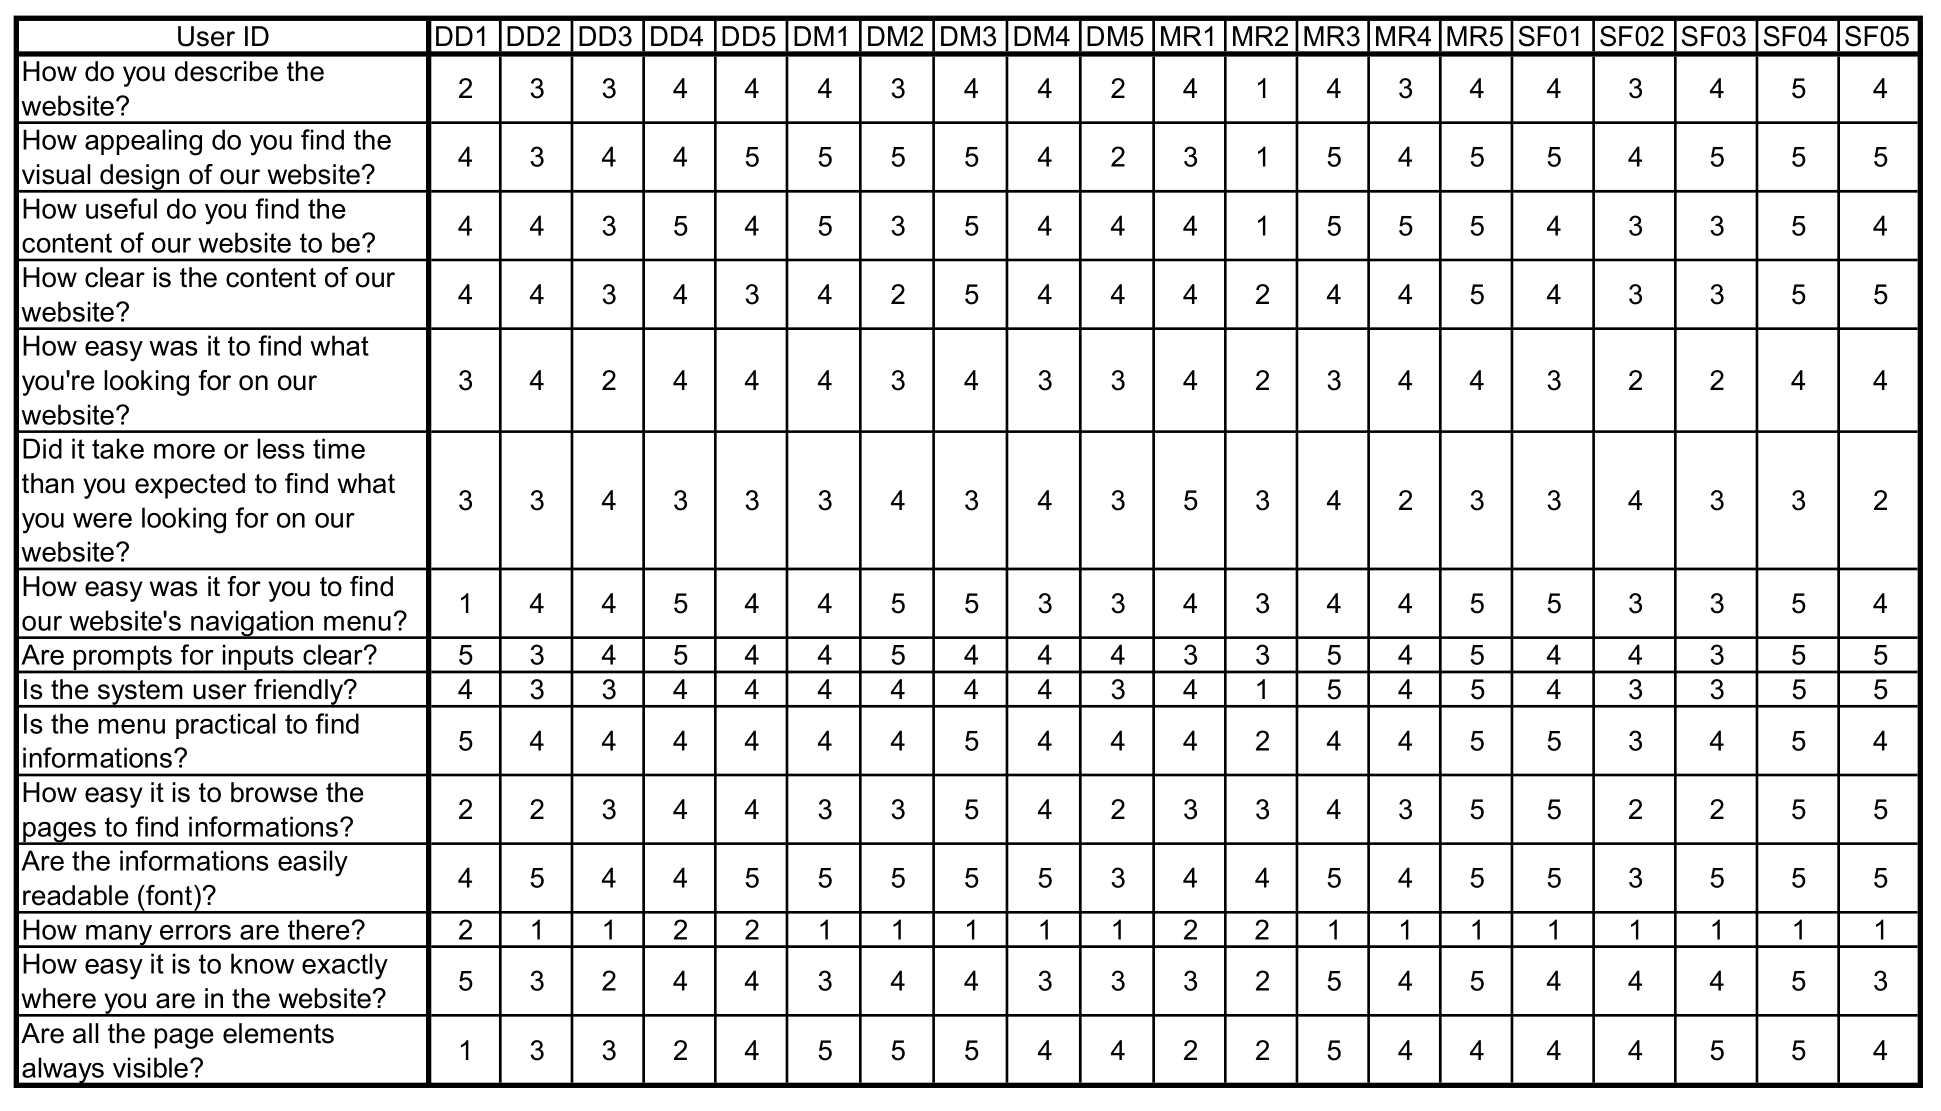
\includegraphics[width=18cm]{images/annex/Questionnaire_answers.png}
        \caption{Questionnaire user answers}
        \label{fig:my_label}
    \end{figure}
    \begin{figure}[H]
        \centering
        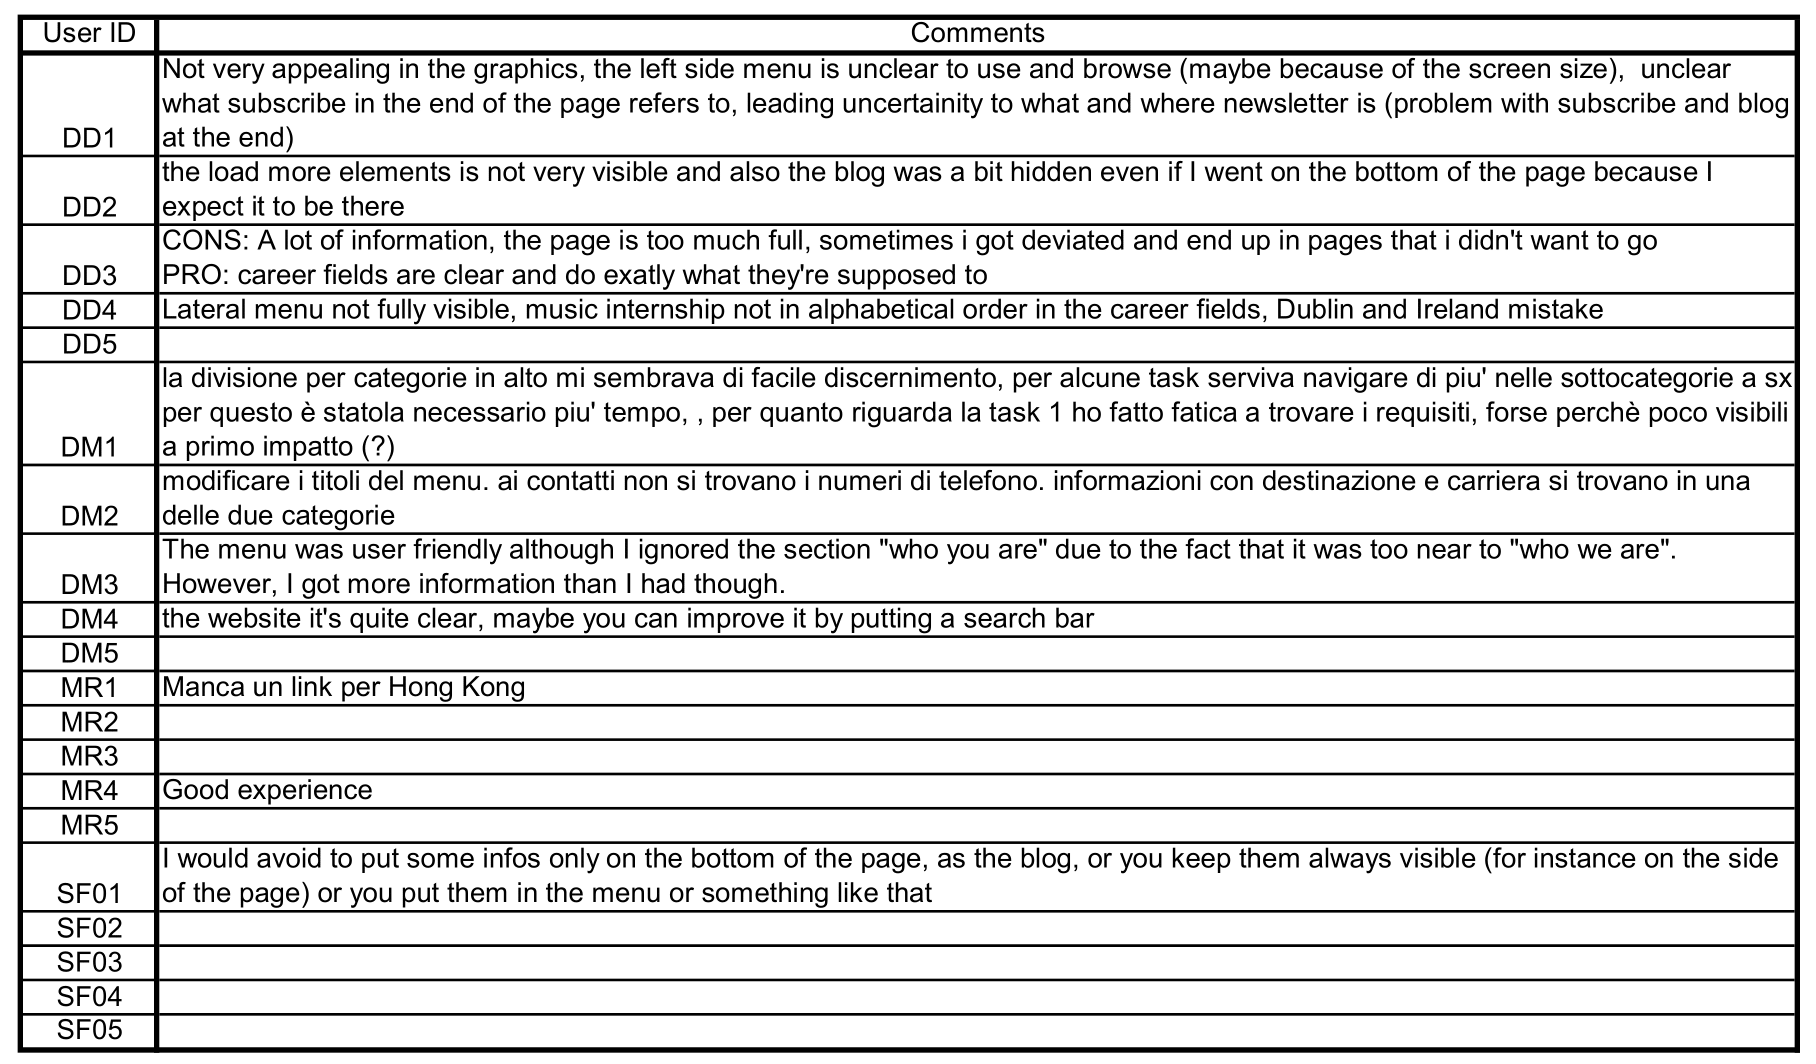
\includegraphics[width=18cm]{images/annex/Questionnaire_comments.png}
        \caption{User comments}
        \label{fig:my_label}
    \end{figure}


%%%%
\end{document}